\documentclass[a4paper,12pt,oneside]{book}
\renewcommand{\baselinestretch}{1.5} 
\usepackage{amsfonts}
\usepackage{amssymb}
\usepackage{amsmath}
\usepackage{mathtools}
\usepackage{latexsym}
\usepackage{amsthm}
\usepackage{graphicx}
\usepackage[USenglish,magyar]{babel}
\usepackage{t1enc}
\usepackage[utf8]{inputenc}
\usepackage{color}
\usepackage{fancybox}
\usepackage{anysize}
\usepackage{lmodern}
\usepackage{fix-cm}
\usepackage{mathcomp}
\usepackage{float}
\usepackage{gensymb}
\usepackage{subcaption}
\usepackage{wasysym}
\usepackage{array}
\usepackage{nccmath}
\usepackage{multirow}
\usepackage{enumitem}
\usepackage[bottom]{footmisc}
\usepackage{setspace}
\usepackage{textgreek}
\usepackage{listings}
\usepackage{fancyhdr}
\usepackage{blindtext}
\usepackage{hyperref}
\usepackage[table,xcdraw]{xcolor}


\hypersetup{colorlinks=true,
linkcolor=black,
urlcolor=blue}

\newcolumntype{P}[1]{>{\centering\arraybackslash}p{#1}}

\marginsize{3cm}{2.5cm}{2.5cm}{2.5cm}

\setlength{\headheight}{14.5pt}
\makeatletter
\newcommand{\figcaption}{\def\@captype{figure}\caption}
\newcommand{\tabcaption}{\def\@captype{table}\caption}
\makeatother
\usepackage{footnote}
\makesavenoteenv{tabular}
\newcommand{\nev}{Szabó Ferenc}
\newcommand{\neptun}{JODV94}
\newcommand{\cim}{FPGA-s EEPROM programozó eszköz tervezése}

\fancypagestyle{plain}{
    \fancyhf{} % Clear header and footer for plain style
    \fancyhead[L]{\cim} % Left-aligned header text
    \fancyhead[R]{\neptun} % Right-aligned header text
    \fancyfoot[C]{\thepage} % Centered page number in the footer
}

\pagestyle{fancy}
\fancyhf{} % Clear all header and footer fields
\fancyhead[L]{\cim} % Left-aligned header text
\fancyhead[R]{\neptun} % Right-aligned header text
\fancyfoot[C]{\thepage} % Centered page number in the footer


\begin{document}

%\frontmatterf
\thispagestyle{empty}

\begin{center}
		\textsc{\Large{Miskolci Egyetem}}
	
	\begin{figure}[H]
		\centering
		
\includegraphics[scale=0.5]{misk_egy.png}
	\end{figure}
	
	\textsc{\Large{Gépészmérnöki és Informatikai Kar}}\\	
	\vspace{5mm}	
	\textsc{\Large{Automatizálási és Infokommunikációs Intézet}}\\
	
	\vspace{14mm}	
	\textbf{\Large{\cim}}\\
	
	\vspace{10mm}
	\textsc{Készítette:}\\
	\textbf{\nev}\\
	\vspace{20mm}
	
	%\textsc{Tervezésvezető:}\\
	%\textbf{Tervezésvezető neve}\\
	%beosztása\\
	\vspace{5mm}
	\textsc{Konzulens:}\\
	\textbf{Konzulens neve}\\
	beosztása\\
	%\vspace{5mm}
	%\textsc{Konzulens:}\\
	%\textbf{Konzulens neve2}\\
	%beosztása
	
	\vspace{35mm} Miskolc, 2025.	
	
\end{center}
\thispagestyle{empty}
\clearpage
\thispagestyle{empty}
\begin{center}
	\textsc{\Large{Eredetiségi Nyilatkozat}}
\end{center}
{\setstretch{1.5}
Alulírott \textbf{\nev}; Neptun kód: \textit{\neptun} a Miskolci Egyetem Gépészmérnöki és Informatikai Karának végzős, \textit{gépészmérnök} szakos hallgatója ezennel büntetőjogi és fegyelmi felelősségem tudatában nyilatkozom és aláírásommal igazolom, hogy
\begin{center}
	\cim
\end{center}
című szakdolgozatom/diplomatervem saját, önálló munkám; az abban hivatkozott szakirodalom felhasználása a forráskezelés szabályai szerint történt.

Tudomásul veszem, hogy szakdolgozat esetén plágiumnak számít:
\begin{itemize}
	\item 	szószerinti idézet közlése idézőjel és hivatkozás megjelölése nélkül;
	\item	tartalmi idézet hivatkozás megjelölése nélkül;
	\item	más publikált gondolatainak saját gondolatként való feltüntetése.	 
\end{itemize}
Alulírott kijelentem, hogy a plágium fogalmát megismertem, és tudomásul veszem, hogy
plágium esetén szakdolgozatom visszautasításra kerül.\\
Miskolc, \today


{\raggedleft\vspace{1cm}(\textit{\nev})
	
}
}

\mainmatter

\clearpage
\tableofcontents
\listoffigures
\listoftables
\iffalse
\chapter{Jelölésjegyzék, indexek}
\textit{\textbf{Latin betűvel jelöltek:}}
\begin{table}[H]
	\centering \renewcommand{\arraystretch}{1.2}
	\begin{tabular}{p{2cm}p{6cm}p{4cm}}
		a&Állandó&-\\
		A& Állandó&-\\
		A&Felület&m$^2$\\
	\end{tabular}
\end{table}
\textit{\textbf{Görög betűvel jelöltek:}}
\begin{table}[H]
	\centering \renewcommand{\arraystretch}{1.2}
	\begin{tabular}{p{2cm}p{6cm}p{4cm}}
		$\alpha$&Hőátadási tényező&$\text{W}/\text{m}^2\text{K}$\\
		$\varepsilon$&Porozitás&-\\
		
	\end{tabular}
\end{table}
\fi

\chapter{Idegen nyelvű összefoglaló}
Here comes the summary...


\chapter{Bevezetés}
\section{Téma választás Háttér}
Szinte naponta hallhatunk újabb és újabb, egyre gyorsabb és hatékonyabb Intel illetve AMD hagyományos desktop processzorokról. Ugyanakkor létezik egy másik típusú integrált áramkör, amelyről kevesebb szó esik, mégis számos területen meghatározó szerepet játszik: ezek az FPGA-k. 

Az FPGA-k széles körben alkalmazottak. Az FPGA-k egyik legnagyobb előnye, hogy lehetővé teszik a mérnökök számára saját, célzottan megtervezett logikai műveletek végrehajtását, rendkívül nagy sebességgel. Nem feltétlenül azért gyorsabbak, mert több GHz-es órajellel rendelkeznek, mint egy mai hagyományos CPU, hanem mert az áramkörök működése nagyon specifikusan, az adott feladathoz igazítva valósítható meg. Egy FPGA-ban akár több százezer ugyanolyan logikai blokkot lehet tervezni és megvalósítani. Emiatt kiválóak lehetnek a párhuzamos számításban. Így minden terület, ahol ez fontos lehet, használva vannak, legalább a fejlesztési szakaszban. 

Például valós idejű rendszerekben vagy bonyolult jelfeldolgozási feladatokban. A mesterséges intelligenciáknál is fontos az ultragyors párhuzamos adat átvitel vagy feldolgozás. Például I/O feladatoknál. De az FPGA-kat jellemzően AI gyorsítók vagy AI processzorok ként is alkalmazzák. Mesterséges intelligencia betanítási feladatokban az FPGA-alapú gyorsítók gyorsabb teljesítményt tudnak nyújtani, mint a hagyományos GPU-k. Hasonló előnyök miatt az FPGA technológia kiemelt szerepet kapott a kép- és videófeldolgozás területén is. Számos fogyasztói elektronikai eszközben, például virtuális valóság szemüvegekben FPGA-k végzik a beérkező videójelek feldolgozását és a kijelzőkre történő leképezését. 

Az automata járművek fejlesztése során is használtak, hiszen alapvető fontosságú a környezet gyors és pontos érzékelése ezeknél a rendszereknél, ami nagymértékű párhuzamos adatfeldolgozást igényel. Jelentős szerepet töltenek be a hagyományos processzorok és az ASIC-ek fejlesztései során. Gyakran vannak használva a tervezők által új dizájnok validálására, debuggolására, mielőtt megrendelik az első prototípusokat egy félvezetőgyártó vállalatól. Bonyolult digitális rendszerek működése gyorsan és költséghatékonyan tesztelhetők, ha FPGA-kon vannak szimulálva. Mindezek alapján elmondható, hogy az FPGA egy olyan technológia, amely meghatározó szerepet tölt be a különböző iparágakban, és várhatóan a jövőben még inkább. 

Tanulmányaim során különösen megfogott ez a terület, ezért választottam szakdolgozatom két fő témájául az FPGA-k és a VHDL hardverleíró nyelv mélyebb megismerését. A projektemben a NYÁK tervezése is kiemelt szerepet kapott. Úgy gondolom, hogy a NYÁK-tervezés mindig is keresett szaktudás marad a villamosmérnöki szakmában, hiszen bármilyen modern beágyazott rendszer létrehozása elképzelhetetlen megfelelő áramköri integráció nélkül. 

A jövőben szeretnék beágyazott rendszerek fejlesztésével foglalkozni, hol a hardveres és szoftveres ismeretek egyaránt fontosok. A NYÁK-tervezés tudása ebben alapvető kompetenciának számít.

A szakdolgozat témája, miről szól(?), mi a célkitűzés(?), a szakdolgozat felépítése (?) mi az egyes fejezetek rövid tartlama (?)
\section{A Project terv bemutatása}
Projectembe egy összetett, de egyedül megvalósítható beágyazott rendszert akartam megvalósítani. Es használni, illetve próbára szerettem volna tenni a VHDL-ben való tervezési tudásomat. Szerettem volna egy számomra új programozási nyelvel is megismerkedni, és végül a C++-t választottam.

Ezek miatt egy EEPROM programozó megvalósítását választottam. A project saját ötlet volt, és úgy gondolom megfelelő szakmai kihívás volt.
\begin{figure}[H]
	\centering
	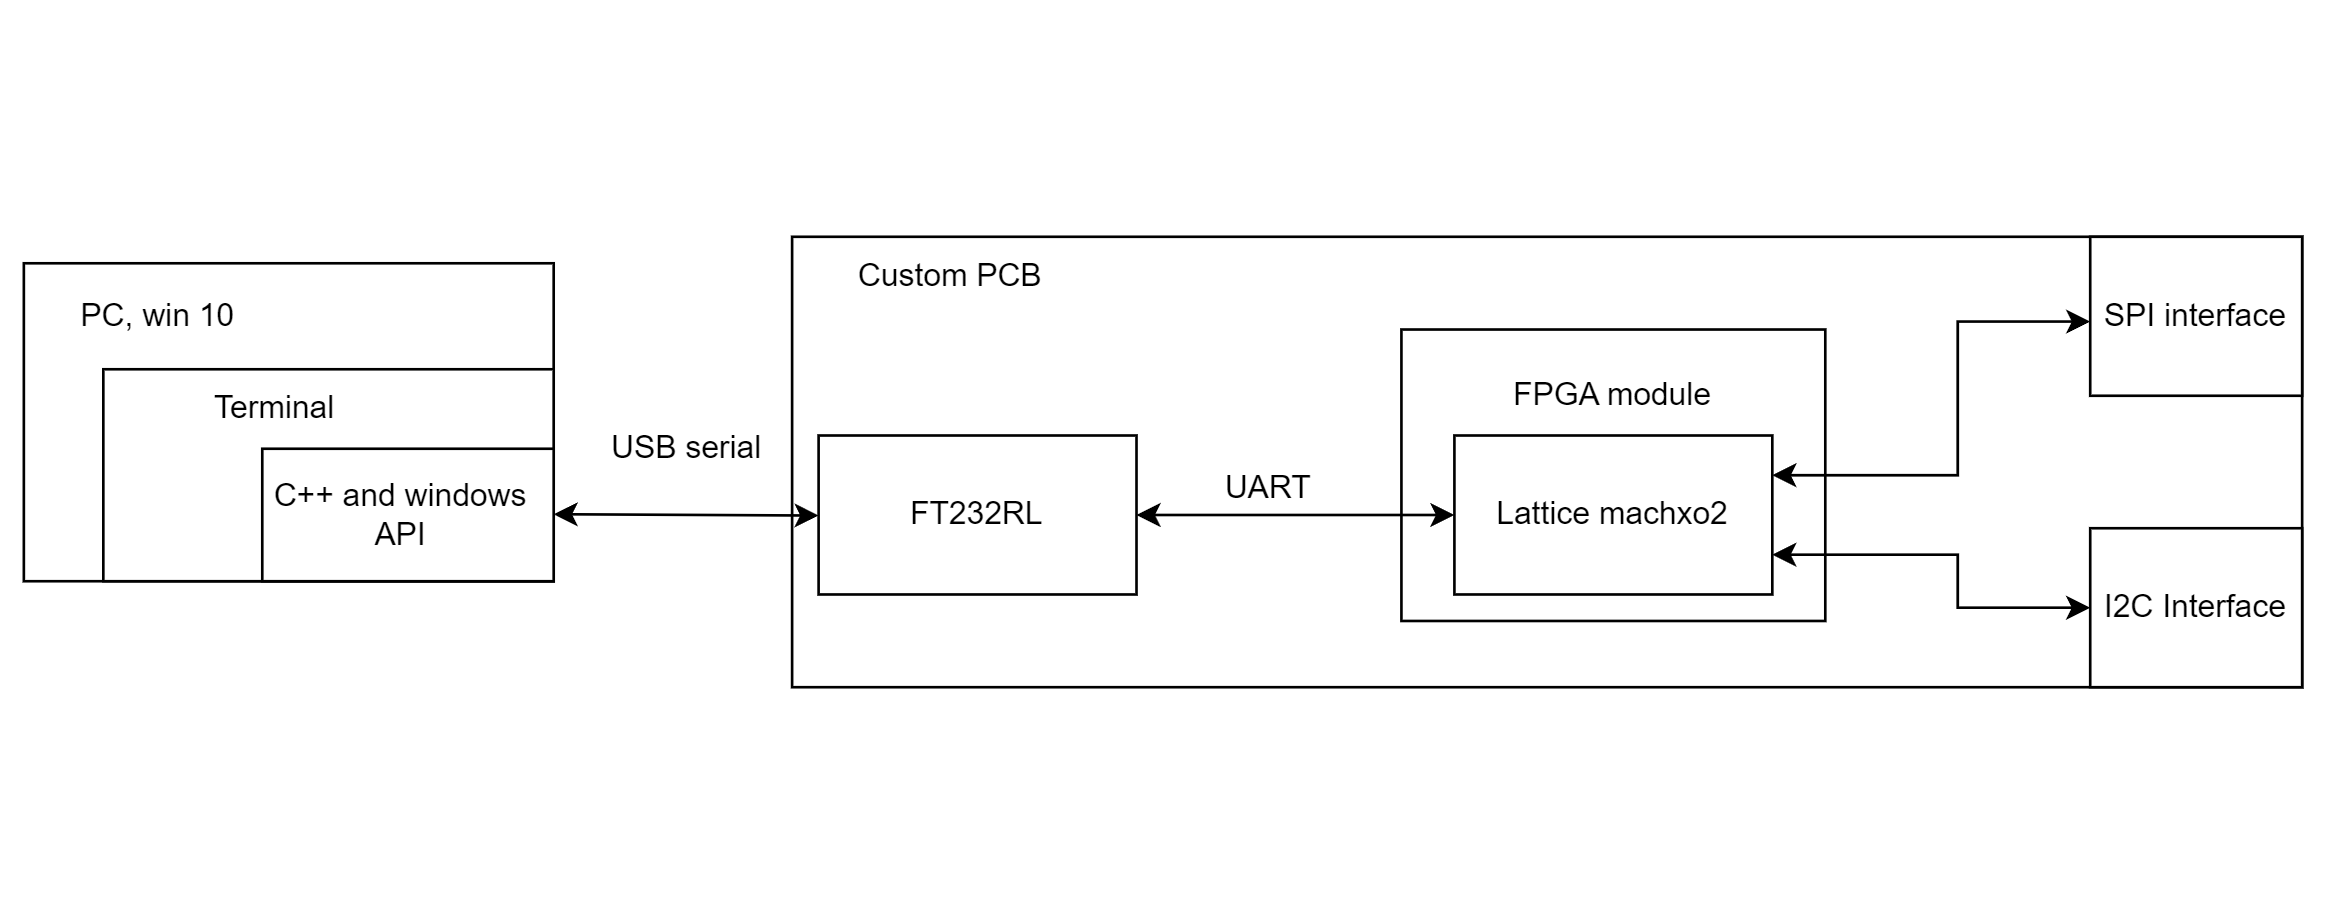
\includegraphics[trim=1mm 1mm 1mm 1mm,scale=0.245]{terv1.png}
	\caption{Projekt terv blokkvázlata}
	\label{Projekt terv}
\end{figure}
Ez a block diagramm volt a project kiinduló ötlete. A felhasználó a c++-ban írt program fútatásával tud kommunikálni a programozóval terminálon keresztül. A programtól kapott  USB kommunikációt a FT232RL váltja át UART csomagokká az FPGA module számára. Az FPGA module-ön megvalósított VHDL-ben megírt logikai áramkör pedig a kapott parancsok alapján küld SPI és I2C parancsokat a programozandó EEPROM chipnek. Az EEPROM chip válaszait esetleges válaszait pedig visszakonvertálja UART csomagokké a FT232RL-nek, amely visszaküldi a PC-nek.
\chapter{Tartalmi rész}

\section{Analízis képek magyarázata és az analízis elrendezés}
A projekt során egy logikai analizátort sokat használtam. A logikai analizátor egy olyan eszköz, amely lehetővé teszi a digitális jelek időbeli viselkedésének megfigyelését és elemzését. Az analizátor képes rögzíteni és megjeleníteni a digitális jelek állapotát, lehetővé téve a tervezők számára, hogy megértsék a rendszer működését és hibáit. Rendkívül hasznos volt debug-olásra.

A Diplomamunkában sok képet használok, amit egy 24MS/s-es OEM logikai analizátorral rögzítettem. Használtam 2 memória module-t is, egy I2C EEPROM-ot meg egy SPI Flash-t is, hogy tudjam ellenőrizni programozó működését.

A I2C EEPROM cikkszáma: AT24C256. Egy 256Kb-es EEPROM \cite{EEPROM}

A SPI Flash cikkszáma W25Q64FV. Egy 64Mb-es Flash \cite{FLASH}

A készített rögzítések Logic nevezetű applikációval vannak vizualizálva és így fognak kinézni:
\begin{figure}[H]
	\centering
	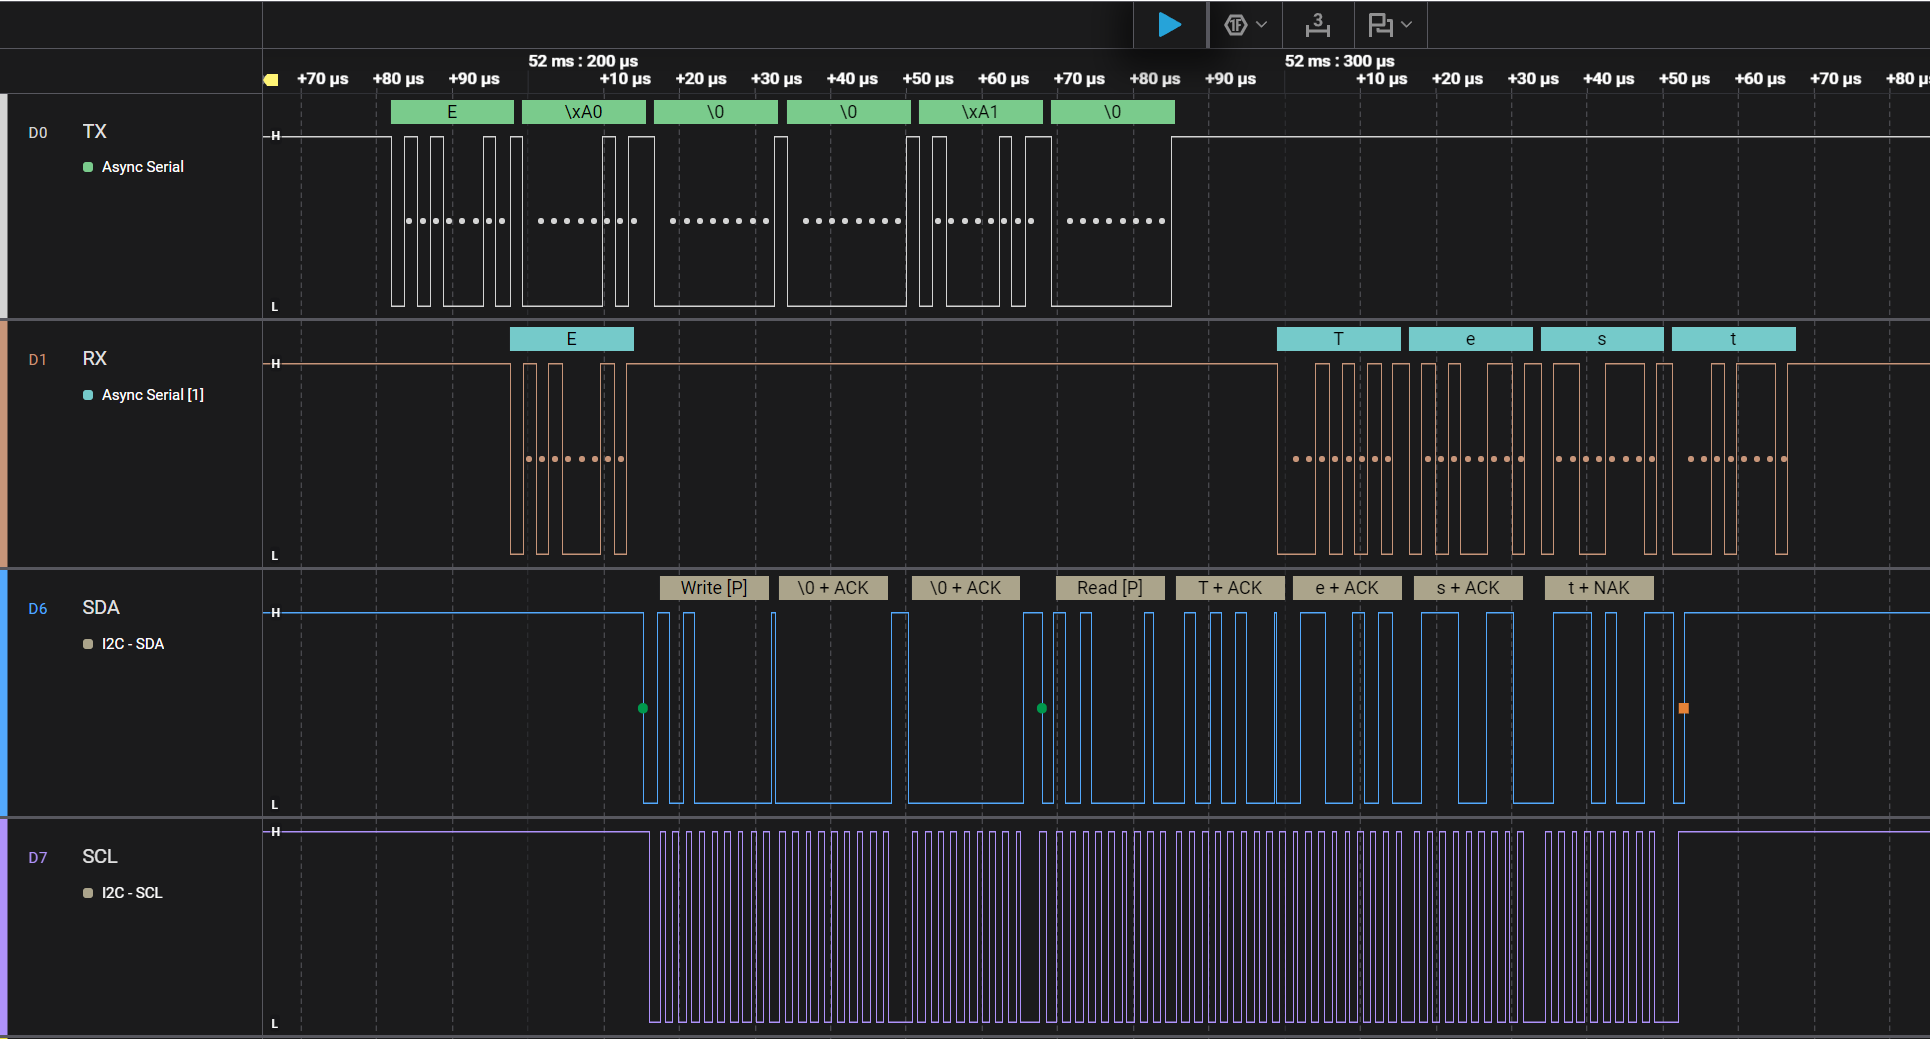
\includegraphics[trim=1mm 1mm 1mm 1mm,scale=0.3]{i2c small read.PNG}
	\caption{Vizalizált analizátor rögzítés példa}
	\label{Vizalizált analizátor rögzítés példa}
\end{figure}

A rögzítésekhez a mérési elrendezés breadboard-on történt, mert a NYÁK-on nem tudom egyszerre csatlakoztatni a memória module-okat meg az analizátort.

Az elrendezés:
\begin{figure}[H]
	\centering
	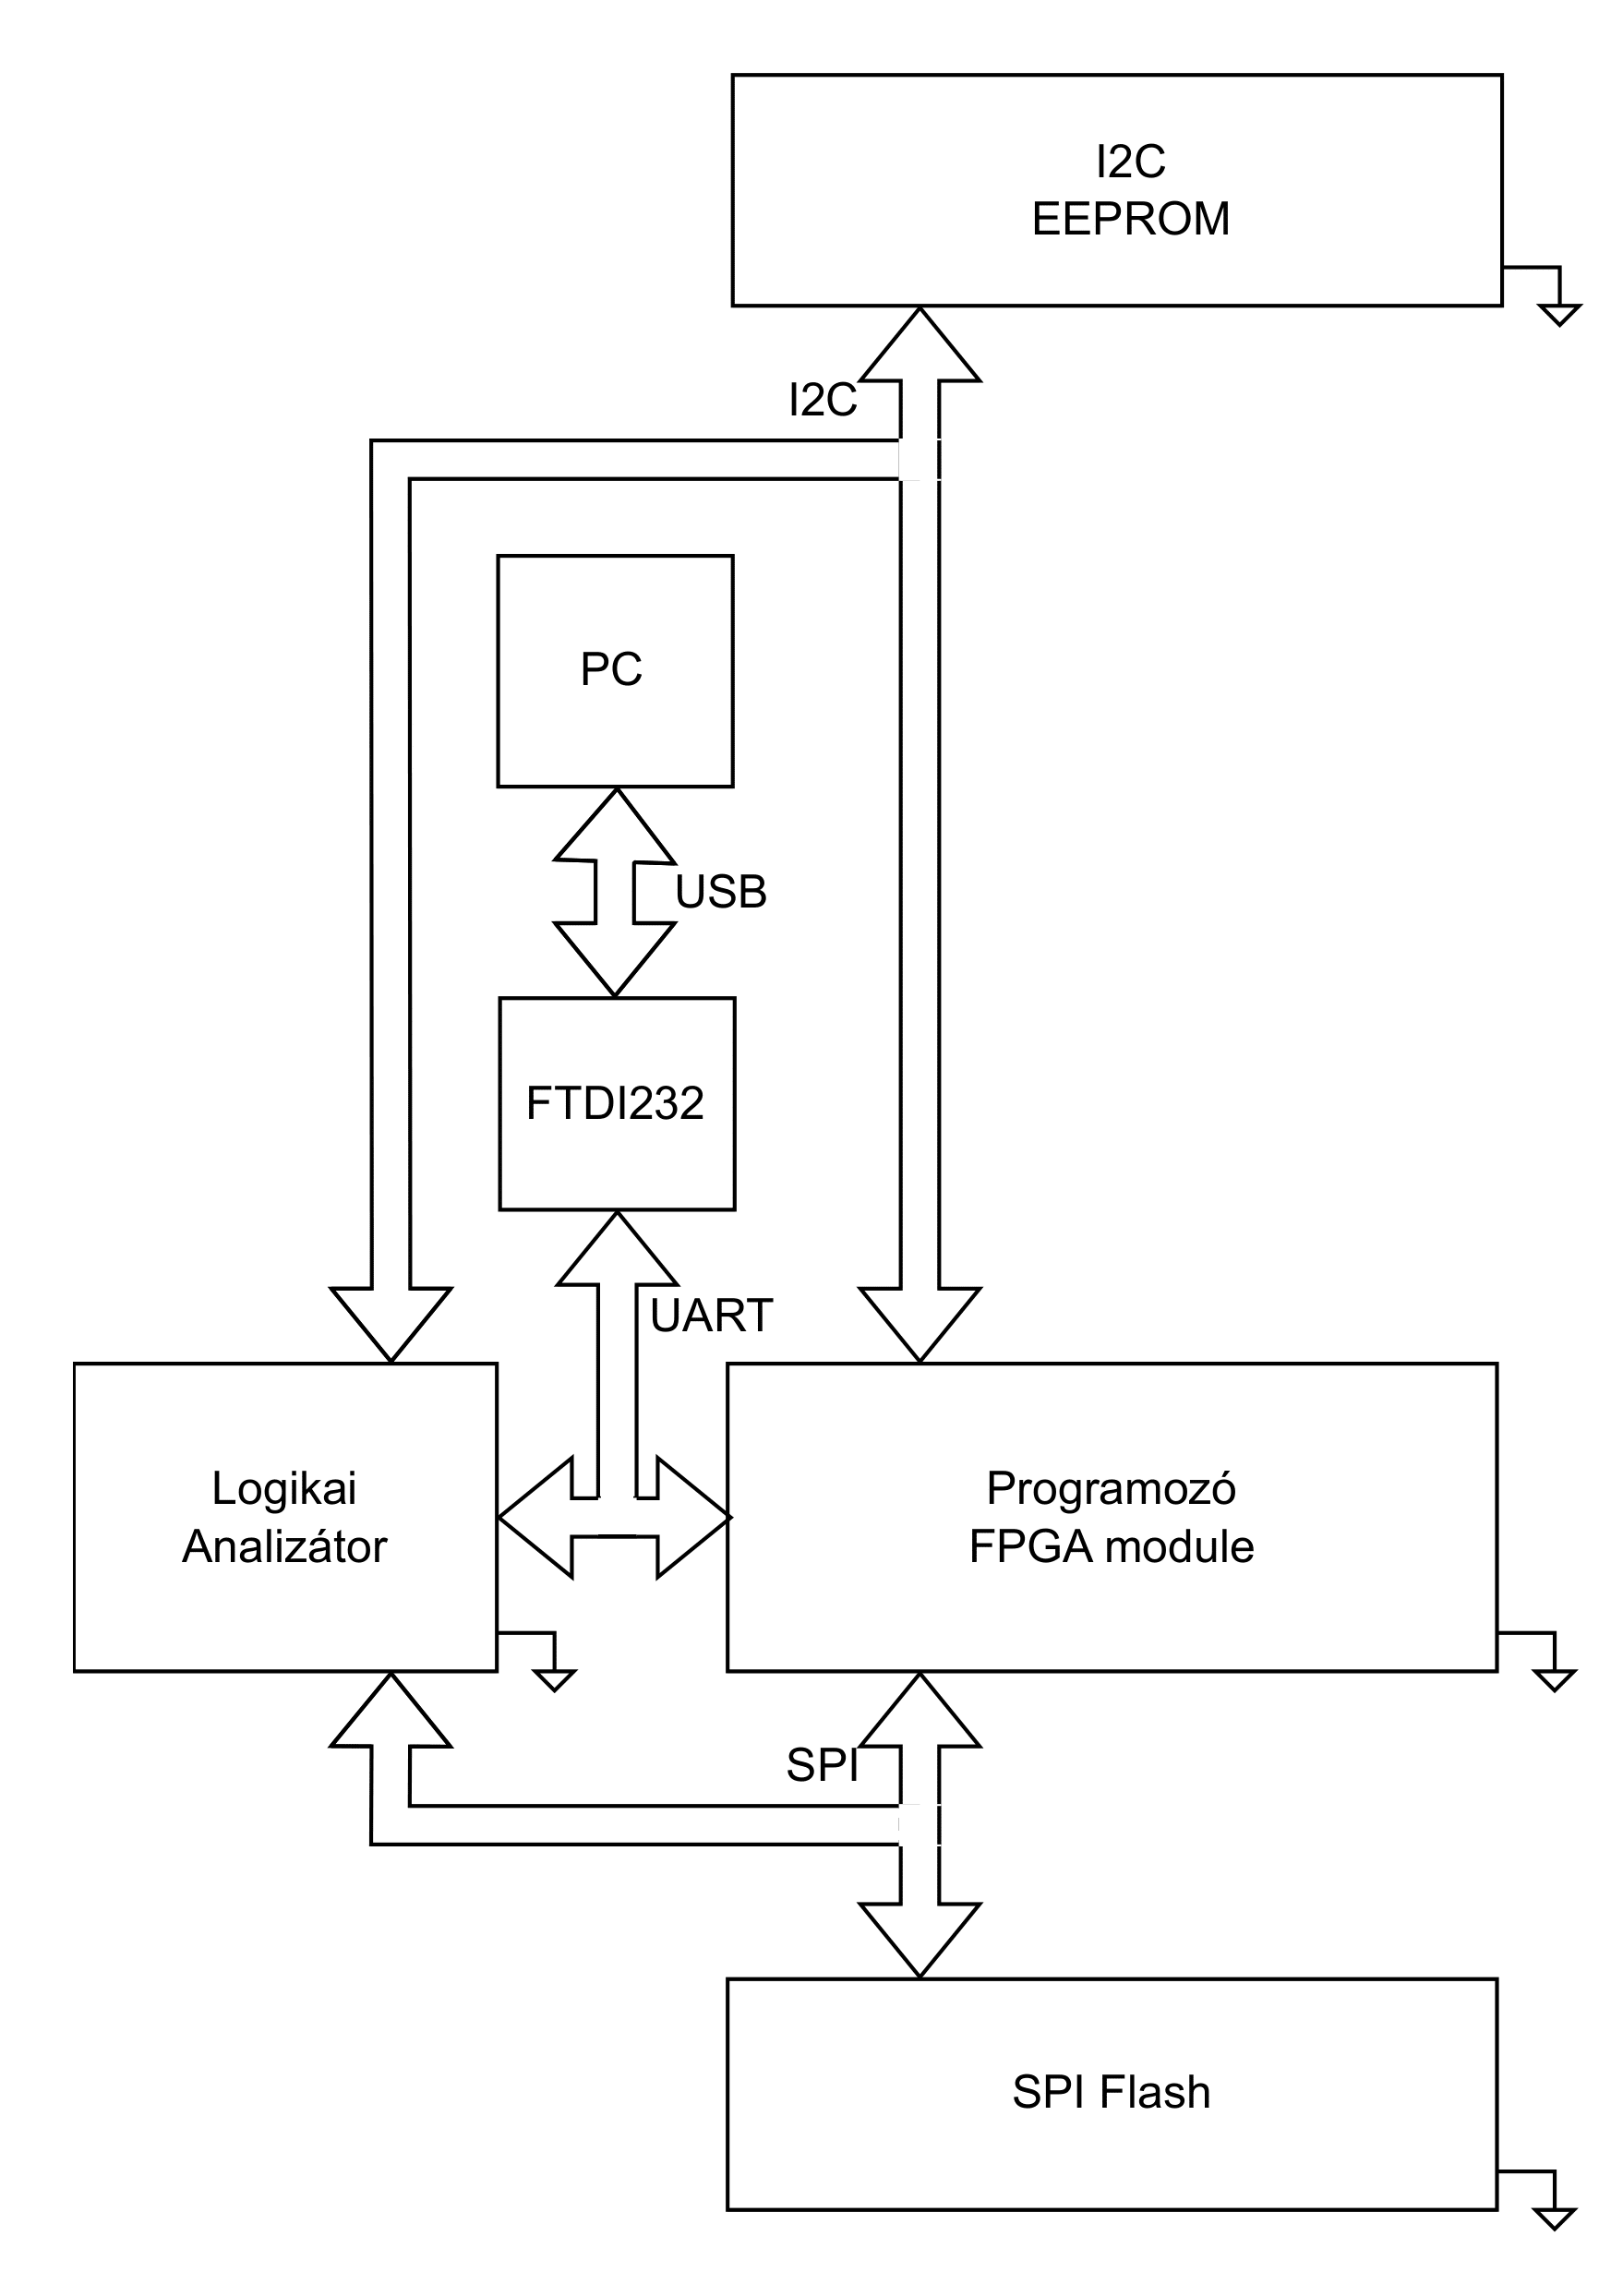
\includegraphics[trim=1mm 1mm 1mm 1mm,scale=0.3]{setupblock.PNG}
	\caption{Analízis elrendezés blokkvázlata}
	\label{Analízis elrendezés blokkvázlata}
\end{figure}
\begin{figure}[H]
	\centering
	\includegraphics[trim=1mm 1mm 1mm 1mm,scale=0.21]{setupreal.PNG}
	\caption{Analízis elrendezés breadboardon}
	\label{Analízis elrendezés breadboardon}
\end{figure}

\section{Technicai Hátter}
\subsection{Mi a FPGA?}

A FPGA egy rövidítés, teljes nevükön ezeket a chipeket, Field-programmable gate array-ként, magyarul a felhasználás helyén programozható logikai kapumátrixokként ismerjük. Az FPGA-ra HDL nyelveken lehet tervezni digitális áramköröket, amik megvalósulnak fizikailag a chip belsejében. 

Az FPGA-k tartalmaznak logikai cellákat, különböző tartalmakkal: flip-flop-ok, LUT-ok, illetve logikai kapuk stb. Ezeket a cellákat lehet programozás során tetszőlegesen összeköttet-ni, így alakulnak ki a tervezett digitális áramkörök. Az FPGA-kon „futó kódot”, azaz a designt, firmwarenek szoktuk nevezni. A firmware szónak más az eredete, mégpedig a csak olvasható memóriába írt program, de az FPGA-k használata körül is elterjedt. A szó maga jól leírja, hogy a FPGA programozható, de közben egy tényleges digitális áramkör valósul meg.

Az FPGA-k megtalálhatók fogyasztói termékekben is, de nagy szerepet játszanak, sok fejlesztési környezetben is, főleg ASIC fejlesztésnél. Termékekben azért lehet hasznos egy FPGA, mert specifikus feladatokat nagyon jól tud elvégezni, és ha a gyártó cég akar változtatni a chip működésén, akkor van rá lehetőség egy firmware frissítéssel. Jó példa az FPGA-k használatára a fogyasztói virtuális valóság készülék. A készülékbe küldött videó adatot fel kell dolgozni, és helyesen rátérképezni a készülék kijelzőire. Mindezt minél gyorsabban, hogy a felhasználó minél kevesebb jelkésést érezzen a fejmozgatás és a kép változása között. Ilyen feladatokra tökéletes az FPGA, hiszen ugyanazt a matematikai műveleteket kell elvégezni, ugyanolyan formátumú adatra, több milliószor egymás után. Egy hagyományos CPU ugyan-ebben a feladatban, rosszabbul szerepelne, még ha hasonlóan gyors az órajele is. A CPU-k arra vannak tervezve, hogy minél több használati esetet fedjenek le, és sok feladat elvégzésére könnyen lehessen őket programozni. Az ilyen feladatoknál éppen emiatt, nem a legoptimálisabban végzik el a számitásokat, mivel nem erre lettek tervezve. Egy példán keresztül bemutatva: ha egy ember kap egy utasítássort kenyérsütéshez, akkor végre tudja hajtani az utasításokat, és képes egy kenyeret sütni, de lassabban, mint egy kenyérsütéshez tervezett automata gép. Ugyanennek az embernek írhatunk utasításokat egy villanykörte becsavarására is, de a kenyérsütő gép soha nem lesz képes villanykörtét becsavarni. Ehhez egy másik gépet kellene tervezni. A hasonlatban az ember egy CPU, az utasítássor a hagyományos kód és a tervezett automata gép egy FPGA-n megvalósított design.

A legtöbb fejlett FPGA manapság SRAM-alapú. Ezek az eszközök konfigurálható logikai blokkokat (CLB-k), és programozható I/O blokkokat tartalmaznak, a jelek chipbe történő be- és kivezetéséhez, valamint programozható útválasztó mátrixot, a CLB-k összekapcsolásához. Ahogy az elnevezés is sugallja, ezeknek az eszközöknek a konfigurációját, a belső SRAM tárolja a chipen. Mivel a programozható összeköttetések nem ideálisak (ellenállásuk és kapacitásuk van), az egyes útvonalak hossza, nagy hatással van az elkészült design elérhető teljesítményére. Az összekapcsolások okozta késések jelentősek, ezért előfordulhat, hogy nehéz megjósolni a sebességet a tényleges útválasztás befejezése előtt. Ahogy az eszközök kihasználtsága megközelíti a 100\%-ot, az útválasztás jelentősen nehezebbé válik. A netlist generáló folyamat, kritikus fontosságú az elkészült design kívánt teljesítményének eléréséhez. Ebben a fejlettebb szintetizátorok nagyban segíthetnek. 

\begin{figure}[H]
	\centering
	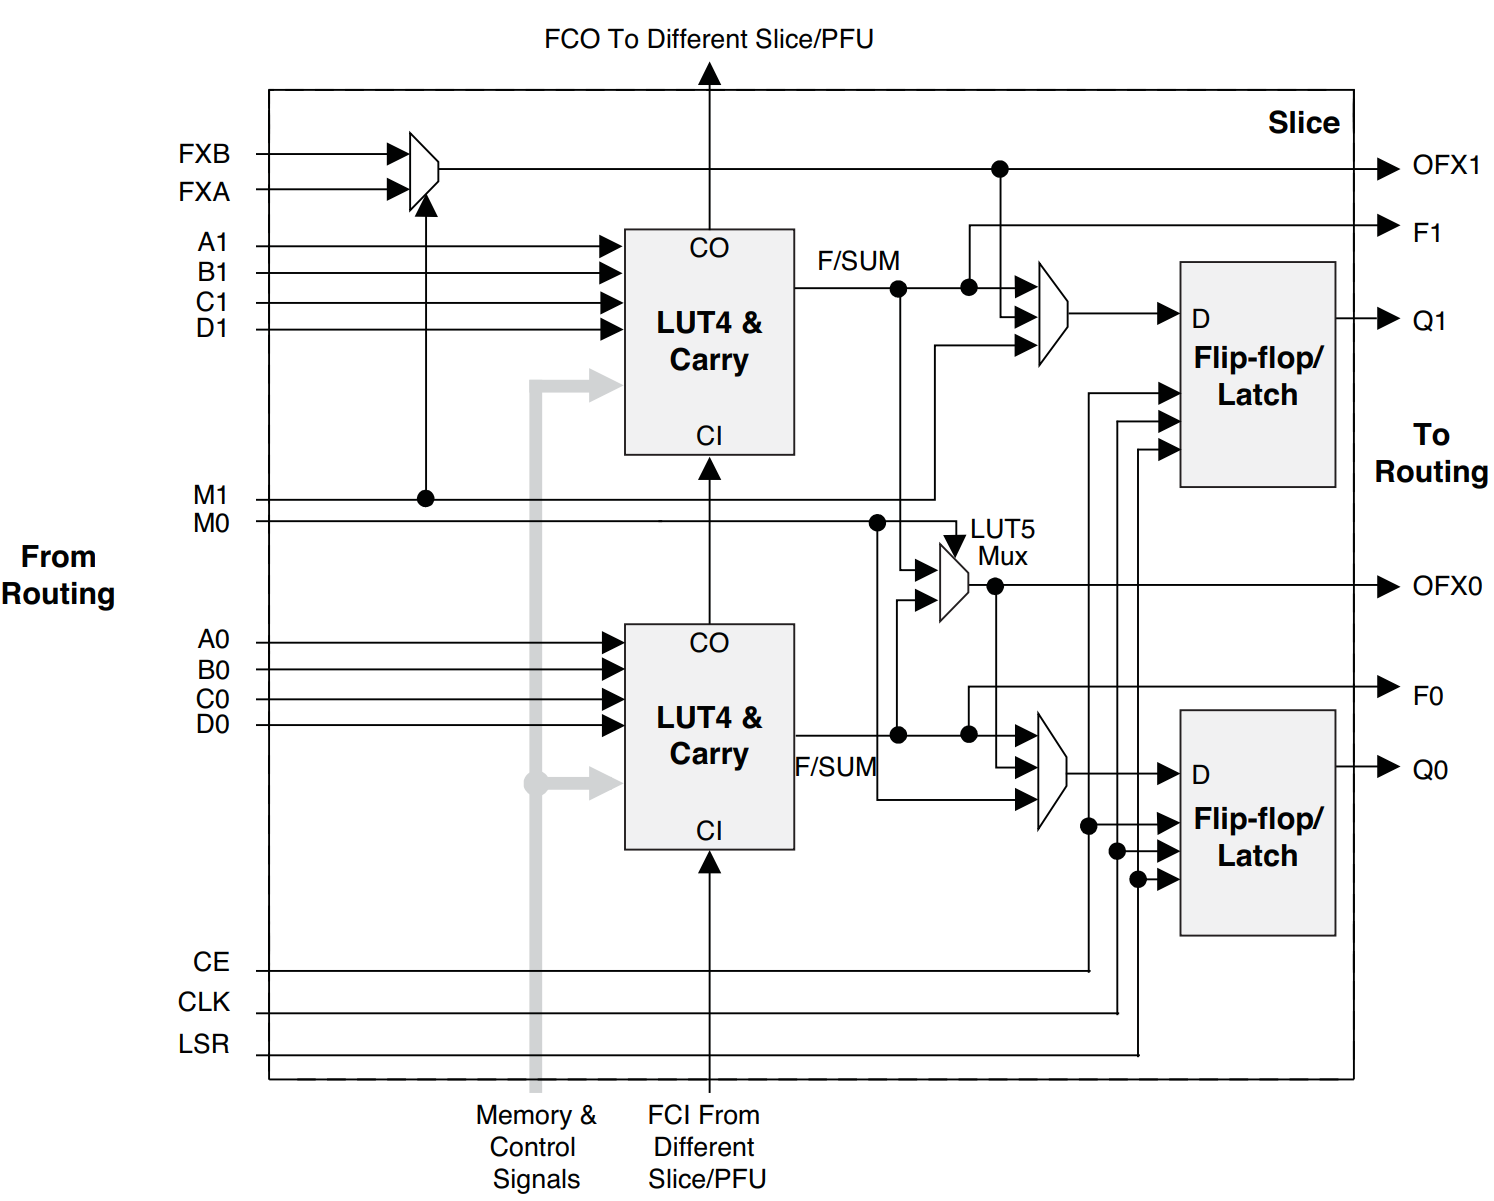
\includegraphics[trim=1mm 1mm 1mm 1mm,scale=0.38]{logickblockfromx02.png}
	\caption{A MAchXO2 FPGA családból egy CLB \cite{fpgaadatlap}}
	\label{CLB}
\end{figure}

A fenti diagram egy egyszerű konfigurálható logikai blokkot / logikai elemet mutat be. Ez a CLB, a MachXO2 FPGA termékcsalád adatlapjában található, ehhez a termékcsaládhoz tartozik az az FPGA is, amivel én dolgoztam. A modern és komolyabb FPGA-k bonyolultabb megvalósításokat tartalmaznak további erőforrásokkal, például blokk RAM-okkal, shift regisz-terekkel, összeadókkal stb. A kis LUT-ok (általában 4-6 bemenet) a kombinációs logika meg-valósítását szolgáljak. A logikai blokkok általában tartalmaznak LUT-okat és néhány flip-flop-ot. A CLB-n belüli kapcsolatok meglehetősen rövidek, így a késleltetésük általában jelentéktelen. A CLB-ket általában az FPGA-n belül szigetekként helyezik el, amelyeket az összekap-csolási mátrix vesz körül, ahol a szomszédos CLB-k, általában rövid és gyors kapcsolatot tar-talmaznak közöttük. Ezen kapcsolatok alkalmazásával bonyolultabb funkciók is megvalósítha-tók, a szomszédos blokkokból történő erőforrások „kölcsönvételével”. Ez azonban, csak meg-felelő elhelyezés mellett történhet meg. Például egy összeadó bitjeit, sorrendben egymás mellé kell helyezni. Ez a szintetizátor felelőssége, de általában a tervezőnek ismernie kell a cél FPGA belső architektúráját, az erőforrások legjobb kihasználása érdekében. Manapság eléggé elter-jedtek a beépített oszcillátorok, tápegységek, melyek a rendszerszintű tervezést segítik, és he-lyet spórolnak. Nem szabad figyelmen kívül hagyni azt a tényt, hogy a megfelelő tápegység megtervezése meglehetősen összetett feladat a modern FPGA-k számára, ahol sok jel, nagy frekvencián működik, és több tápsínre van szükség, nagy áramerősséggel. Az indítási blokkok segíthetnek a terv minden részének megfelelő inicializálásában, rendszerindítás után, vagy alaphelyzetbe állítás esetén. 

Az FPGA-kat jelfeldolgozásra is használják, ahol a dedikált szorzók / digitális jelfeldolgozási blokkok hatékonyabbak, mint a CLB-alapú blokkok. Ezek a dedikált blokkok sokkal kevesebb helyet foglalnak el az IC belsőjében, és magasabb frekvencián, kisebb teljesítménnyel tudnak működni. A belső memória flip-flop-okból való szintetizálása, pazarló folyamat. A modern FPGA-k beépített memóriablokkokat tartalmaznak, amelyekre általában szükség van, mivel a legtöbb tervnek valamilyen FIFO-ra, vagy bufferre van szüksége az átmeneti adatok tárolására. A legtöbb FPGA legalább kétportos memóriát tartalmaz, ahol az olvasási és írási műveletek egyszerre történhetnek, két dedikált porton. Az órajelgenerátorok, manapság egy-aránt elterjedt erőforrások.

\subsection{Mi a VHDL?}

A VHDL az egyik legelterjedtebb HDL, a VERILOG mellet. A HDL, azaz hardware description language, magyar neve, hardware leíró nyelv. A VHDL egyben egy standard, és egy programozói nyelv. Programozói nyelv, mert segítségével absztrakt módon lehet leírni egy digitális áramkör működését, amit majd szintetizálás után, meg lehet valósítani egy FPGA segítségével. Egyben egy standard is, amit az IEEE tart fent. Minden 5 év után frissül, hogy lépést tartson az ipari szükségekkel. A VHDL nehézsége, mint minden más leíró nyelvnek is, nem csak az, hogy meg kell tanulni a programozó nyelvet, hanem az is, hogy tudni kell, hogy a különböző szerszámok, amiket használunk a fejlesztés során, hogyan értelmezik majd a kódot. Amikor egy design működik szimulátorban, nincs rá garancia, hogy szintetizálás után is működni fog. Komolyabb designok tervezése ezeket a lépéseket szokta követni:
\begin{enumerate}[label=(\alph*)]
	\item Az elvárt digitális működés leírása HDL nyelven, egyben, majd a szimulációhoz szükséges „testbench” megírása.
	\item A design szimulálása szimulátorral, debug-olás.
	\item A design szintetizálása a tényleges a FPGA-ra. 
\end{enumerate}
A testbench szerepe az, hogy szimuláció közben, a design bemeneteit szimulálja, illetve kimeneteire válaszoljon, ha kell. Például egy I2C mester tervezése után, a testbench viselkedhet úgy, mint egy szolga. A VHDL tartalmaz szintetizálhatatlan részt is, nagyrészt azért, hogy testbench írásakor egyszerűbben és gyorsabban lehessen haladni. VHDL-nek azt a részét, ami szintetizálható, RTL-nek (register transfer level) hívjuk.

A szintetizálás az utolsó és legkritikusabb lépés, mielőtt egy működő design-t megvalósítunk. 
\begin{enumerate}
	\item A szintetizátor először generál egy kapu szintű netlist-et. Utána a generált netlist-et rátérképezi a specifikus logikai cellákra az FPGA-ban, flip-flop-okra, look-up table-okra és logikai kapukra stb. 
	\item Ezután készül egy netlist, ami a specifikus FPGA modellre tartozik, a szintetizátor eldönti az összes szükséges cella legjobb elrendezését, összecsatolását. 
	\item Végül következik az időzítés analízis. Komolyabb designoknál fontos a helyes működéshez, hogy adott értékeknél ne legyen nagyobb a „slack”. Ezen azt értjük, hogy egy logikai jel később ér a netlist-ben megadott helyére, mint kellene, és emiatt hibás a design. Ilyesmi akkor történik, ha például egy jel túl sok logikai kapun megy át anélkül, hogy az órajelhez újra időzítve lenne. Ilyenkor a megoldás az, hogy a logikai kapuk közepénél, újra szinkronizáljuk a jelet egy flipfloppal.
	\item Ezután a szintetizátor előállít egy bit fájlt, amit rá lehet programozni az FPGA SRAM-jébe.  
\end{enumerate}
A VHDL entitás, egy darab hardware-nek lehet mondani, aminek definiált kimenetei is bemenetei vannak. Egy tervezett entitás lehet komplex, egyszerű, lehet szimpla ÉS kapu vagy akár SPI mester is. Egy entitáson belül lehet több, már megtervezett entitás is összekapcsolva. 

Egy entitásnak két része van, amit VHDL-ben meg kell tervezni: 
\begin{enumerate}
	\item Az entitás definíció, ahol meg kell adni az entitás nevét, bemeneteit és kimeneteit
	\item A szerkezet definíció, ahol az entitás működését kell leírni. 	  
\end{enumerate}

\subsection{Kommunikációs protokollok}
Ahhoz, hogy adatot tudjunk átadni egy feladótól egy fogadónak, fontos, hogy ugyanazt a „nyelvet” beszéljék. Ha két ember különböző nyelven beszél egymással, akkor nem fogják egymást érteni. Ehhez hasonlóan, ha egy feladó IC, az adatot egy bizonyos protokoll szerint kódolja, de a fogadó nem ismeri a protokollt, akkor nem történik meg az adatátvitel. Tehát egy protokoll szabályai leírjak az adat kódolását/dekódolását, és a csatornát is, amin folyik a kommunikáció. 

\subsubsection{UART}
Az általam készített programozó sok kommunikációs protokollt használ, köztük az UART-ot. A számítógéppel való kommunikálás UART-on keresztül történik, a FTDI232 UART-USB átalakító segítségével.

Az UART egy rövidítés teljes neve: Universal asynchronous receiver transmitter. Egy aszinkron, soros protokoll, ami azt jelenti, hogy nincs órajel vonal, hanem az időzítést a küldő és fogadó külön-külön követi, és az adatot bitenként kell küldeni/fogadni. Ezért fontos, hogy mindkét fél ugyanazzal az időzítéssel dolgozzon. Ezt az időzítést szimbólum per szekundumban mérjük, és Baud-nak hívjuk. Ha a kommunikáció időzítése 9600 Baud, akkor a fogadó tudja, hogy egy szimbólum 1/9600 másodpercig lesz megtartva a vonalon, és helyesen tudja mintavételezni az adatkeretben levő adatot. De a Baud ráta nem egyenlő a maximum adatsebességgel, tehát 9600 Baud az nem 9.6 kb/sec. Ez az adatkeret, és egy pár kötelező időzítés miatt van. Az adatkeret azért szükséges, hogy a fogadó tudja mikor kezdődik egy adat, és hol van a vége. Az adatkeret tartalmazhat egy paritás bitet is. Az adatkeret tulajdonságai is egyezni kell az adó és fogadó között.

Tehát a fontos tulajdonságok:
\begin{itemize}
	\item Baud ráta
	\item Adatbitek száma 
	\item Paritás bit használata.
\end{itemize}
\begin{figure}[H]
	\centering
	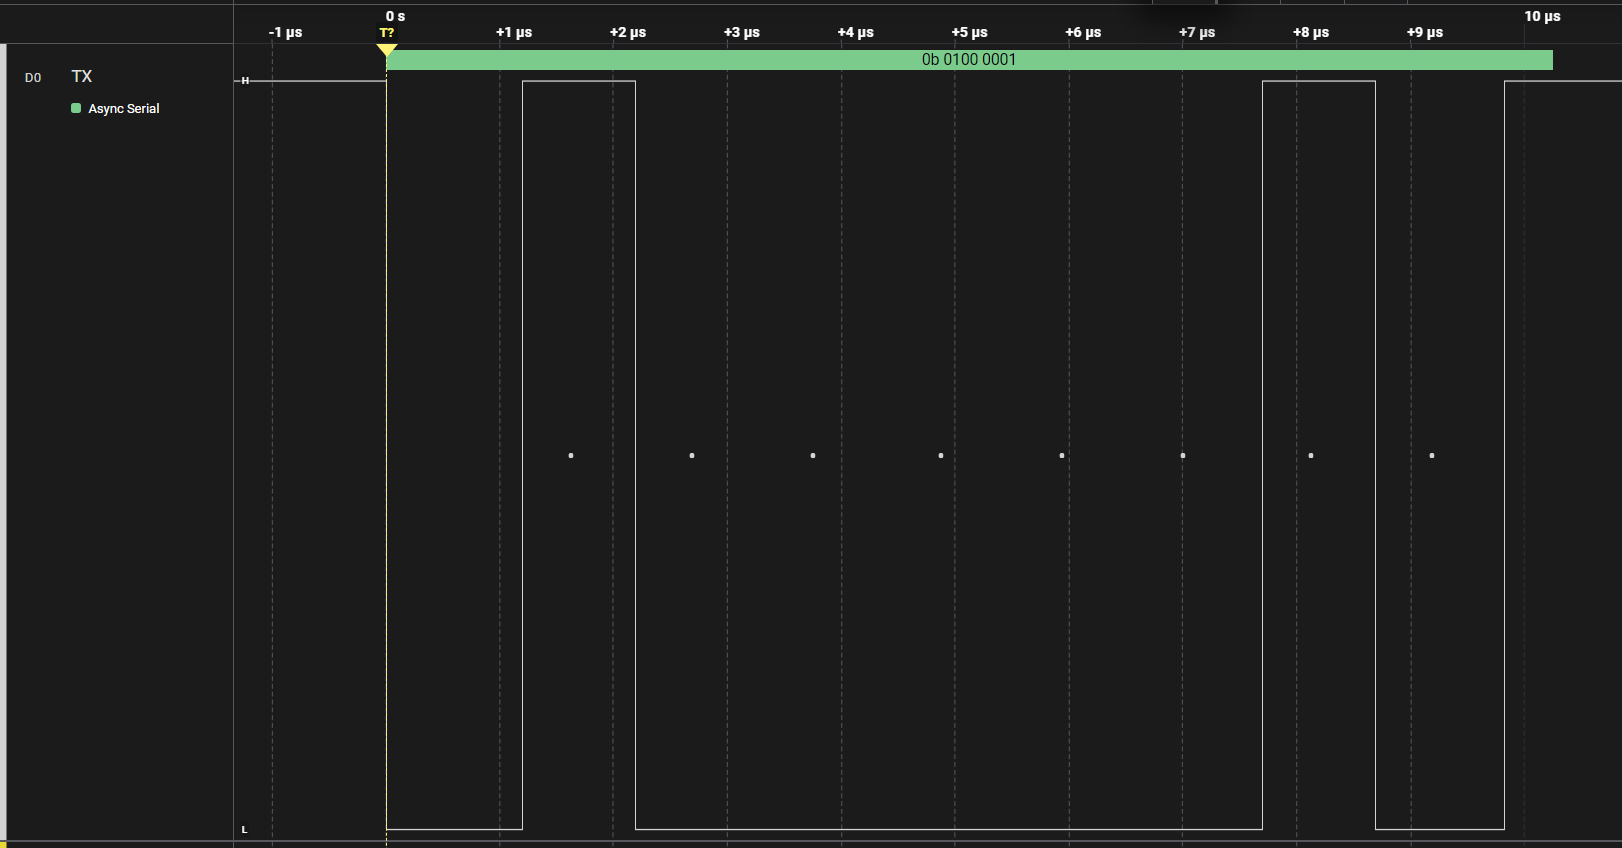
\includegraphics[trim=1mm 1mm 1mm 1mm,scale=0.35]{UARTfromAnalyzer.PNG}
	\caption{UART adatkeret}
	\label{UARTkep}
\end{figure}
A képen látható egy adatkeret, amit az FPGA küld az FTDI232-nak. A Baud ráta ebben az esetben 921600 Baud, azaz egy szimbólum ideje: 1/ 921600 Baud = 1.09 μs. Ezt az analizátor program segítségével meg is jelöltem a képen.

A tétlen állapotot megbontja az indító bit.

Az indító bit után látható az adat bájt LSB bit sorrenddel, ez azt jelenti, hogy az első bit értéke $2^0$ a második $2^1$, stb. 

Ezután látható a stop bit, a stop bit 1 db szimbólum ideéjig magas szinten tartja a vonalat. Ha van paritás bit akkor az a stop bit előtt van volna, én viszont nem használok hiba detektálást.

Ezután a vonal visszatér a tétlen állapotba (logikai magas).
\begin{figure}[H]
	\centering
	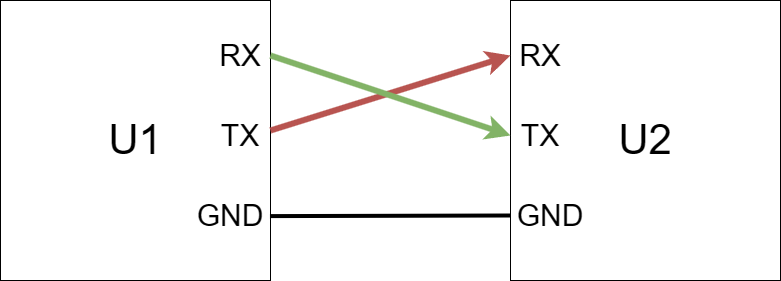
\includegraphics[trim=1mm 1mm 1mm 1mm,scale=0.55]{uartblock.png}
	\caption{UART blokkvázlat}
	\label{UARTblockk}
\end{figure}
Az UART protokollban a vonalakat RX-nek és TX-nek hívjuk. A küldő és a fogató rendelkezik saját RX és TX lábbal. A TX láb a küldő- és a RX láb a fogadó láb. Nem kötelező az összes vonalakat használni, ezért a kommunikáció lehet szimplex, vagy fél/teljes duplex. Szimplex módban, csak az U1 Tx lába csatlakozna, az U2 RX lábához, és csak küldeni lenne képes az adatot. A fél/teljes duplex konfigurációban, hasonlóan lenne kapcsolva a képhez, és attól függően, hogy az U1/U2 képes-e egyszerre küldeni és olvasni adatot, a kommunikáció fél, illetve teljes duplex lenne. Az én nyákomon a kommunikáció teljes duplex.
\subsubsection{SPI}
Az SPI kommunikációs protokoll, egy rendkívül elterjedt és rugalmas protokoll, teljes neve serial peripheral interface. Az UART-al ellentétben szinkronizált protokoll, és teljes duplex.
\begin{figure}[H]
	\centering
	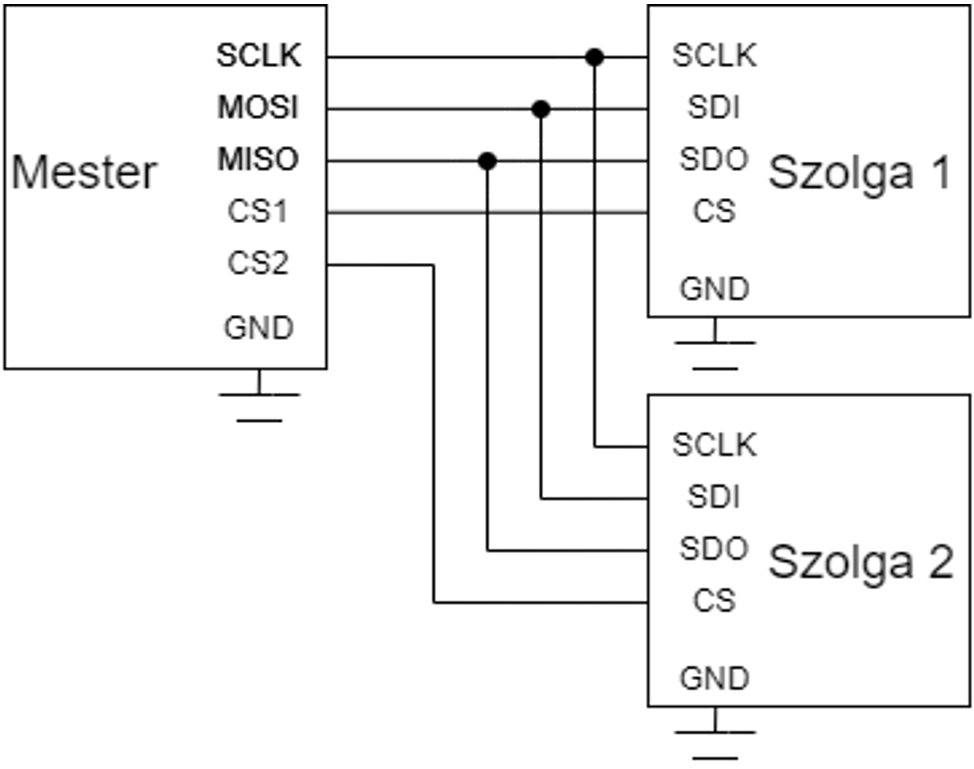
\includegraphics[trim=1mm 1mm 1mm 1mm,scale=0.5]{SPIblockk.PNG}
	\caption{SPI blokkvázlat}
	\label{SPI blokkvázlat}
\end{figure}
SPI protokollban több, mint két IC tudja használni ugyanazokat a vonalakat, de egyszerre csak kettő lehet aktív, ezért van mester és szolga. A mester szerepe az, hogy kiválasszon egy szolgát, és kezdje a kommunikációt. A szolga csak akkor képes kommunikálni, ha ki van éppen választva. A kiválasztást a CS „chip select” vonalokon keresztül végzi el a mester. Minden szolgának külön CS vonal kell, de a többi vonalat meg tudják osztani. Emiatt minden szolgának elég 4 láb (referencia pontot kivéve), még a mesternek kell 3db, plus minden szolgaként egy láb (ismét referencia pontot kivéve). 


Mivel az SPI szinkron protokoll a szimbólum sebességet itt nem az előre beállítót Baud ráta határozza meg, hanem a mester előállít egy órajelet a SCLK vonalon, amit figyelnek a szolgák a kommunikálás alatt. A szimbólumsebesség tehát csak a SCLK frekvenciájától függ. 


A MOSI vonal egy rövidítés. Teljes neve magyarra fordítva „mester ki szolga be”, ez a vonal hordozza a mestertől küldött soros adatot, a szolga oldalán a lábat SDI-nak (soros adat be) hívjuk. A MISO vonal mester be szolga ki és a szolga oldalon SDO-nak (soros adat ki) hívjuk. Az adatkeretet bemutatásához használom ismét a prgramozómat, mégpedig egy kommunikációt egy spi FLASH és az FPGA között.
%%need the thing
\subsection{I2C}
\section{NYÁK tervezés}
\subsection{A NYÁK tevező program bemutatása}
A KiCad egy ingyenes, nyílt forráskódú szoftvercsomag. Elsősorban kapcsolásai rajzok és nyomtatott áramkörök tervezésére szolgál. Egy KiCad projecten belül lehet tervezni nyákokat, kapcsolási rajzokat, lábnyomokat, és szimbólumokat is.

A KiCad sok hasznos segédprogramot is tartalmaz, amelyek segítenek az kapcsolási rajzok és a nyomtatott áramkörök tervezésében. 

Támogatja a kapcsolási rajzok elkészítését, az alkatrészekhez tartozó lábnyomok hozzárendelését, valamint a nyomtatott áramkörök fizikai elrendezésének megtervezését. A PCB tervezés során több réteg kezelésére is lehetőség van, akár 32 rétegű áramkörök tervezése is lehetséges. 

A tervezett áramkörök vizuális ellenőrzését egy integrált 3D nézet segíti, amelyben a felhasználó valósághű képet kaphat a végső NYAK-rol. 

A tervezési folyamat biztonságát a beépített elektromos szabályellenőrző (ERC) és tervezési szabályellenőrző (DRC) rendszerek garantálják, amelyek képesek a gyakori tervezési hibák, például az elmaradt összeköttetések vagy a nem megfelelő távolságok automatikus felismerésére. 

A gyártási előkészítést a KiCad támogatja gyártási fájlok (például Gerber, drill fájlok) generálásával, valamint beépített anyagjegyzék/BOM készítő funkcióval is rendelkezik. Ezen felül a KiCad lehetővé teszi saját szimbólum- és lábnyomkönyvtárak létrehozását, valamint 3D modellek hozzárendelését az alkatrészekhez. 
Amit és is kihasználtam, az, hogy a KiCad szoftver Python szkriptek támogatásával bővíthető, amely különösen hasznos mivel nyílt forráskódú a KiCad. A kiterjedt, közösségi alapú dokumentáció és a hozzáférhető tanulási források tovább növelik a program használhatóságát mind kezdő, mind haladó felhasználók számára. Ezek miatt választottam a KiCad-ot.
\subsection{A KiCad ban végzett munka bemutatása} 
\subsubsection{Kapcsolási rajz}
\begin{figure}[H]
	\centering
	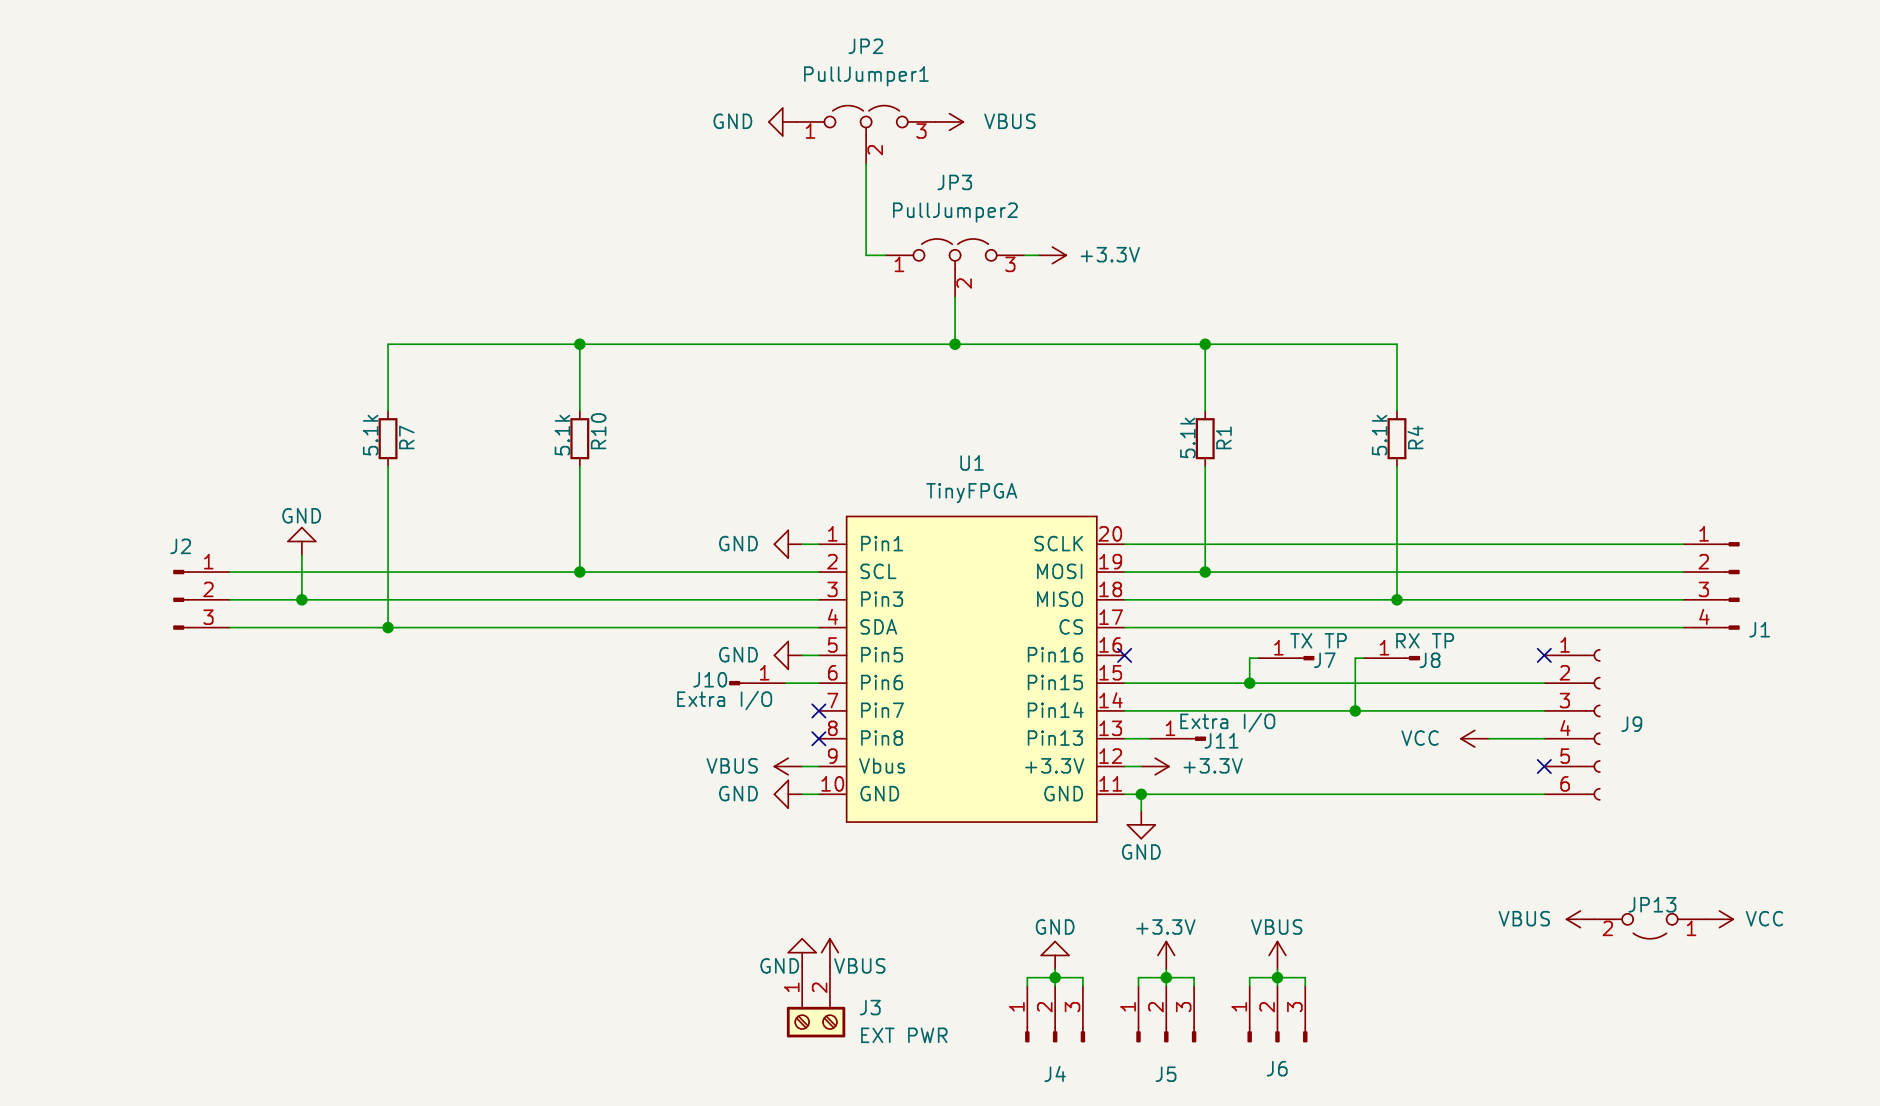
\includegraphics[trim=1mm 1mm 1mm 1mm,scale=0.30]{kapcsolasi rajz.PNG}
	\caption{A programozó kapcsolási rajza}
	\label{teljes kapcsolási rajz}
\end{figure}
A kapcsolási rajz viszonylag egyszerű, nincs sok alkatrész. A felhúzó ellenállásokat kivéve csak csatlakozók meg jumper-ek vannak a NYÁK-on. Mégis igyekeztem sok időt fordítani a tervezésre.

A célom az volt, hogy ez egy általánosan használható EEPROM programozó legyen, ehhez rugalmasnak kellet megterveznem.  A jumper-ek segítségével az ellenélésok 3V3 vagy 5V felhúzó ellenállások, vagy akár lehúzó ellenállások ként is tudnak szolgálni. Így sok féle EEPROM module-okat tud támogatni az áramkőr. Ha a JP2 jumper 1-es és 2-es pin-je van közösítve, akkor a GND van kiválasztva. Ha a JP2 jumper 2-es és 3-es pin-je van közösítve, akkor 5V van kiválasztva. Ha a JP3 jumper 2-es és 3-es pin-je van közösítve, akkor 5V van kiválasztva.
\begin{figure}[H]
	\centering
	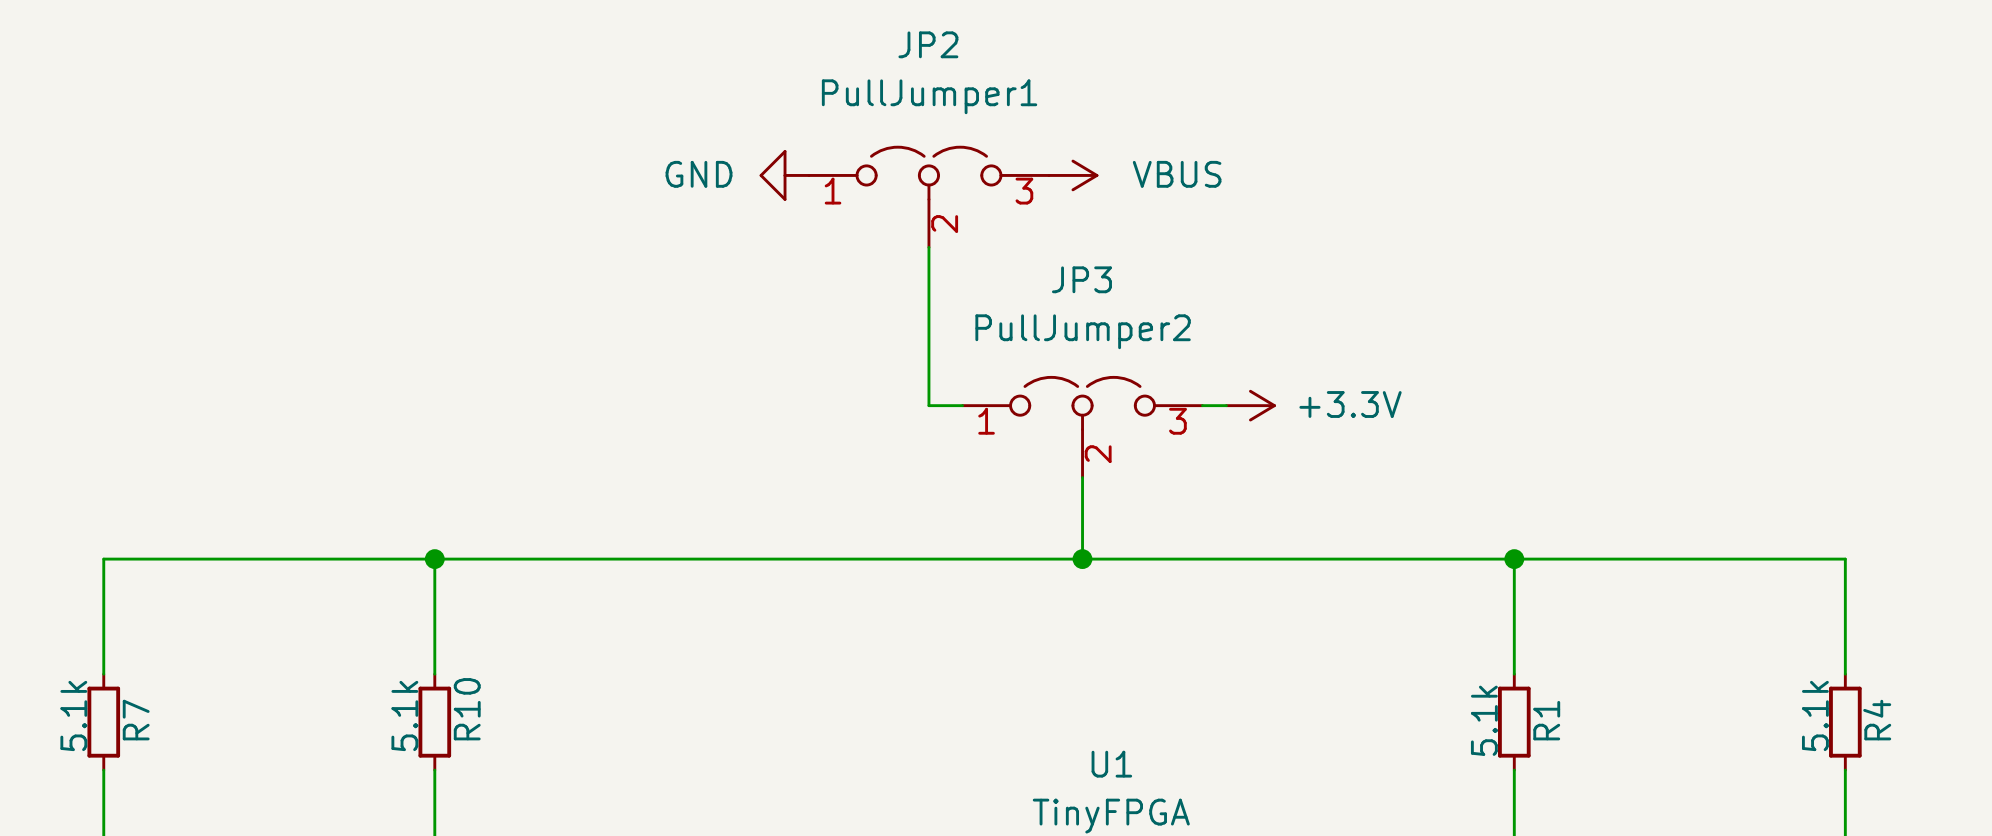
\includegraphics[trim=1mm 1mm 1mm 1mm,scale=0.29]{jumperek.PNG}
	\caption{Ellenállás Jumper-ek}
	\label{Ellenállás Jumper-ek}
\end{figure}
\begin{figure}[H]
	\centering
	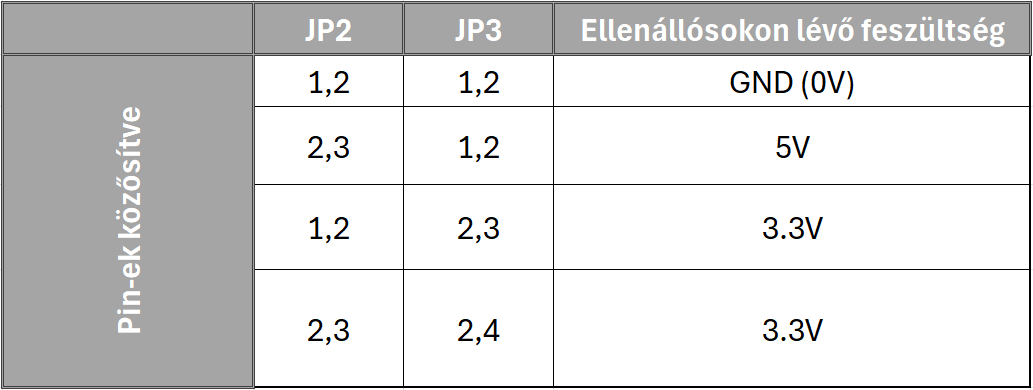
\includegraphics[trim=1mm 1mm 1mm 1mm,scale=0.45]{jumpertable.PNG}
	\caption{Ellenállósokon lévő feszültség összefüggése}
	\label{Ellenállósokon lévő feszültség összefüggése}
\end{figure}
A áramkörnek 4 lehetséges tápja van
\begin{itemize}
	\item A TinyFPGA 5V VBUS PIN-je. A pin közvetlen össze van kötve a module mikró USB 5V tápjával. Tehát amikor a TinyFPGA module csatlakoztatva van a mikró USB-n keresztül a VBUS pin kimenet ként szolgálhat. A TinyFPGA module a betápját is a VBUS látja el. Szóval, ha a TinyFPGA nincs csatlakoztatva az USB-hez akkor a VBUS pin bemenetként is működhet.
	\item A TinyFPGA 3V3 PIN. Ez a kimenet a TinyFPGA module power managment IC-je generálja a VBUS 5V feszültégéből.
	\item Az FTDI232 VCC kimenete. Ami alítható 3V3 és 5V között a FTDI232 module-ön egy jumper-el.
	\item Az EXT PWR csatlakoztatón, amit biztonság kedvéért raktam hozzá az áramkörhöz, ha szükséges lenne a jövőben egy külső táp..
\end{itemize}
A Jumper-ek úgy vannak megtervezve, hogy bármijeik 5V-od bemenet szolgálhasson táp ként a NYÁK-nak meg a hozzá csatolt memória module-oknak. De a tervezett legtöbbet használt konfiguráció az a FTDI232 VCC kimenetét használja az 5V módban. Ilyenkor persze a JP13 jumper két pin-je közösítve kell, hogy legyen, hogy a TINY FPGA megkapja a 5V tápot.
\begin{figure}[H]
	\centering
	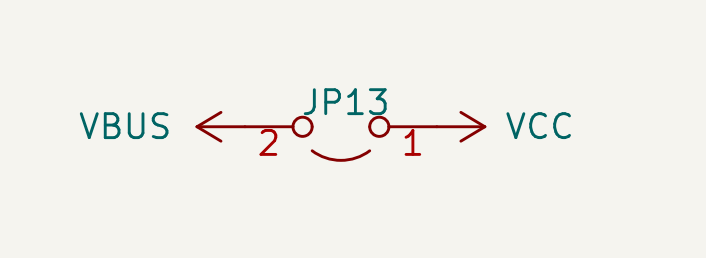
\includegraphics[trim=1mm 1mm 1mm 1mm,scale=0.45]{JP13.PNG}
	\caption{VCC és VBUS közösítő jumper}
	\label{VCC és VBUS közösítő jumper}
\end{figure}
A NYÁK-on ki van vezetve 3-3 pin-en a GND, 3V3, és a VBUS. Ezek a csatlakozok tápként szolgálnak a csatlakoztatott memória module-oknak, illetve merés pontoknak is alkalmasak.
\begin{figure}[H]
	\centering
	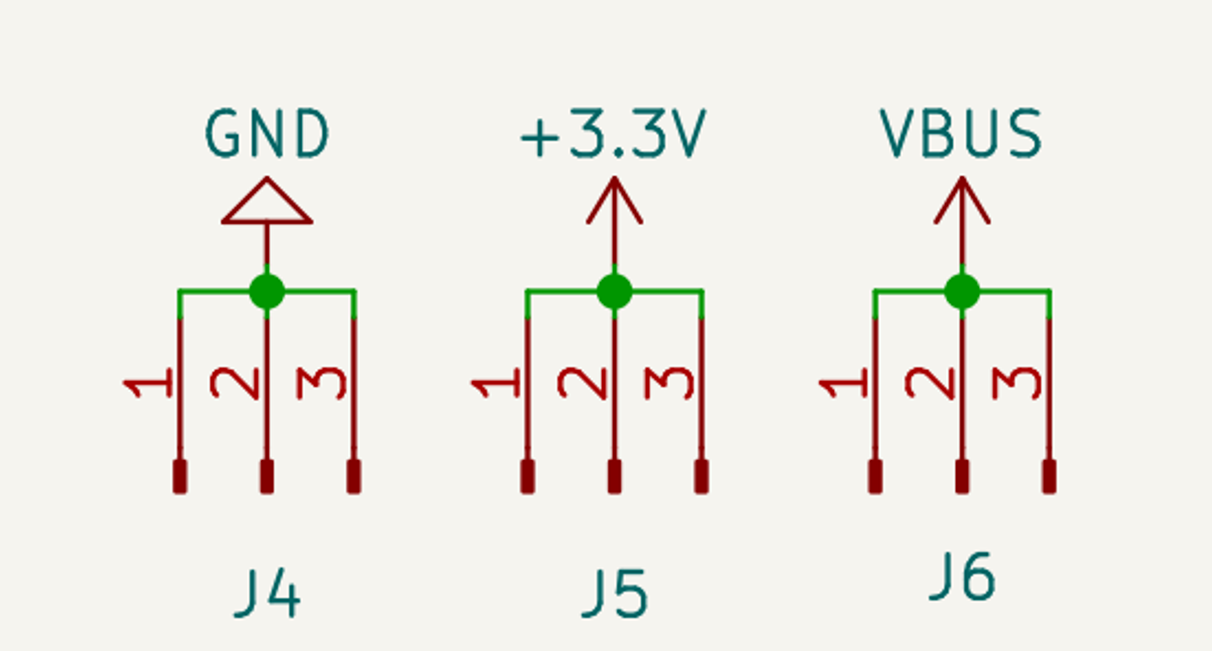
\includegraphics[trim=1mm 1mm 1mm 1mm,scale=0.45]{gnd5v3v3.PNG}
	\caption{Fontos feszültségek és a GND kivezetése}
	\label{Fontos feszültségek és a GND kivezetése}
\end{figure}
\subsubsection{NYÁK tervezés}
\begin{figure}[H]
	\centering
	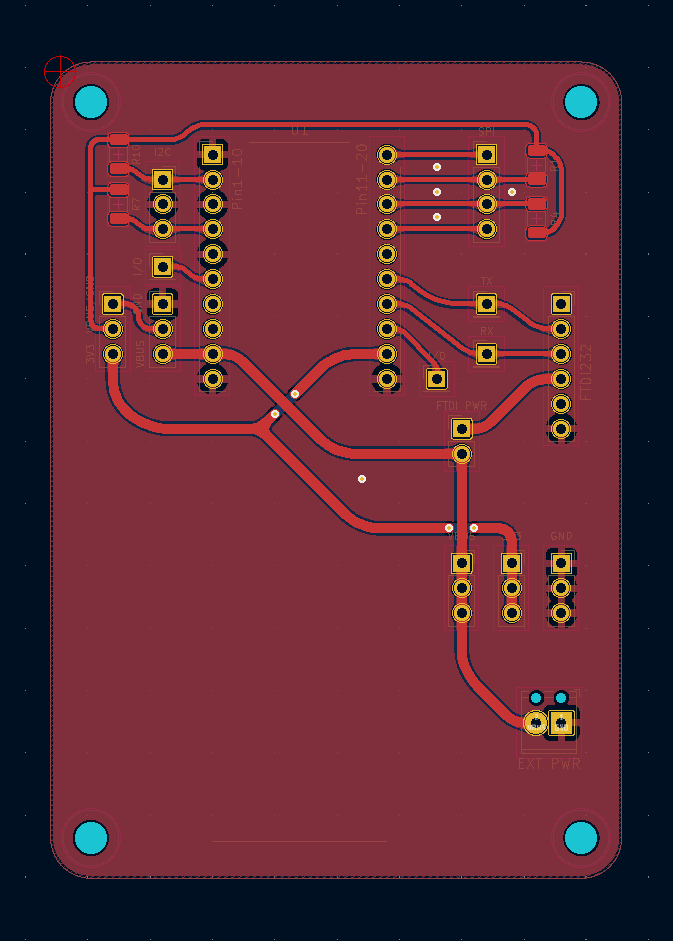
\includegraphics[trim=1mm 1mm 1mm 1mm,scale=0.45]{nyak.PNG}
	\caption{A programozó NYÁK-ja}
	\label{A programozó NYÁK-ja}
\end{figure}
Ez a végleges NYÁK terv, ez az a design, aminek gyártását megrendeltem. Egy két réteges egyszerű nyák. De egy ilyen egyszerűbb NYÁK tervezése közben fontos betartani az alapszabályokat.

Tervezés előtt érdemes beállítani azokat a limiteket, amiket a NYÁK gyártó cég képes gyártani. Ha tudjuk, hogy melyik céget akarjuk használni, akkor a weboldalukon megtalálhatjuk az értékeket. A limiteket a Board Setup funkcióval lehet megadni. Ha jól meg vannak adva az értékek akkor a KiCad nem enged olyan nyákot tervezni, amit nem tud a NYÁK gyártó cég legyártani. Az én esetemben:
\begin{figure}[H]
	\centering
	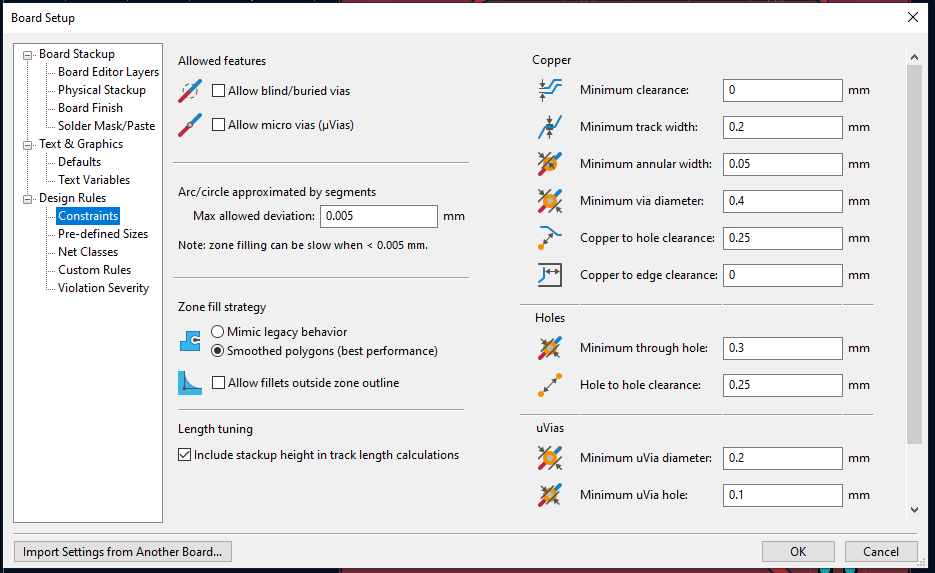
\includegraphics[trim=1mm 1mm 1mm 1mm,scale=0.55]{bosrd limits.PNG}
	\caption{KiCad limit beállítások}
	\label{KiCad limit beállítások}
\end{figure}
\subsubsection{A NYÁK alsó rétege}
A hátsó réteg itt egyszerű. Az egész egy GND réteg, minél kevesebb megszakítással, hogy minimalizálva legzenek az áram visszaútjai, ez ezáltal az arám hurkok területe is.
\begin{figure}[H]
	\centering
	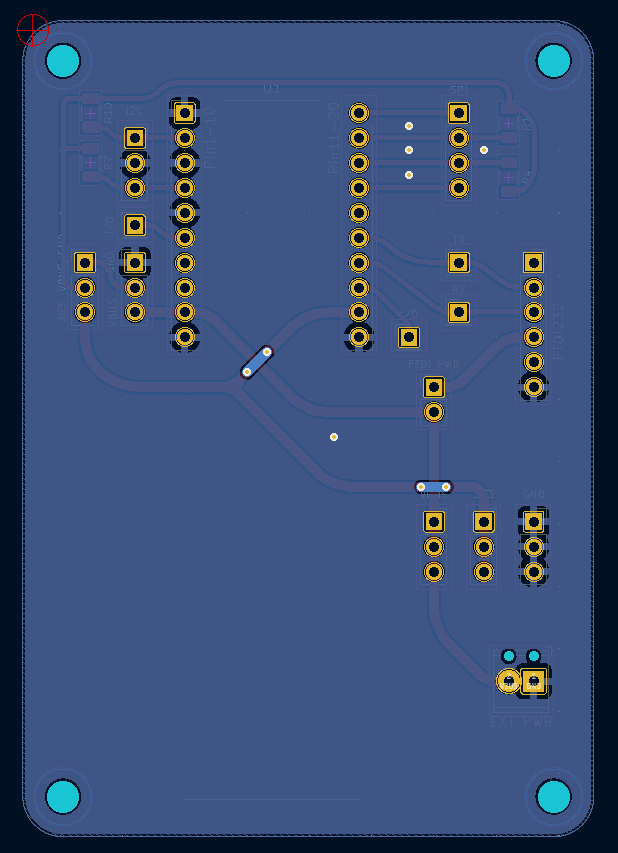
\includegraphics[trim=1mm 1mm 1mm 1mm,scale=0.45]{also reteg.PNG}
	\caption{A NYÁK alsó rétege}
	\label{A NYÁK alsó rétege}
\end{figure}
\subsubsection{Az SPI csatlakozó}
\begin{figure}[H]
	\centering
	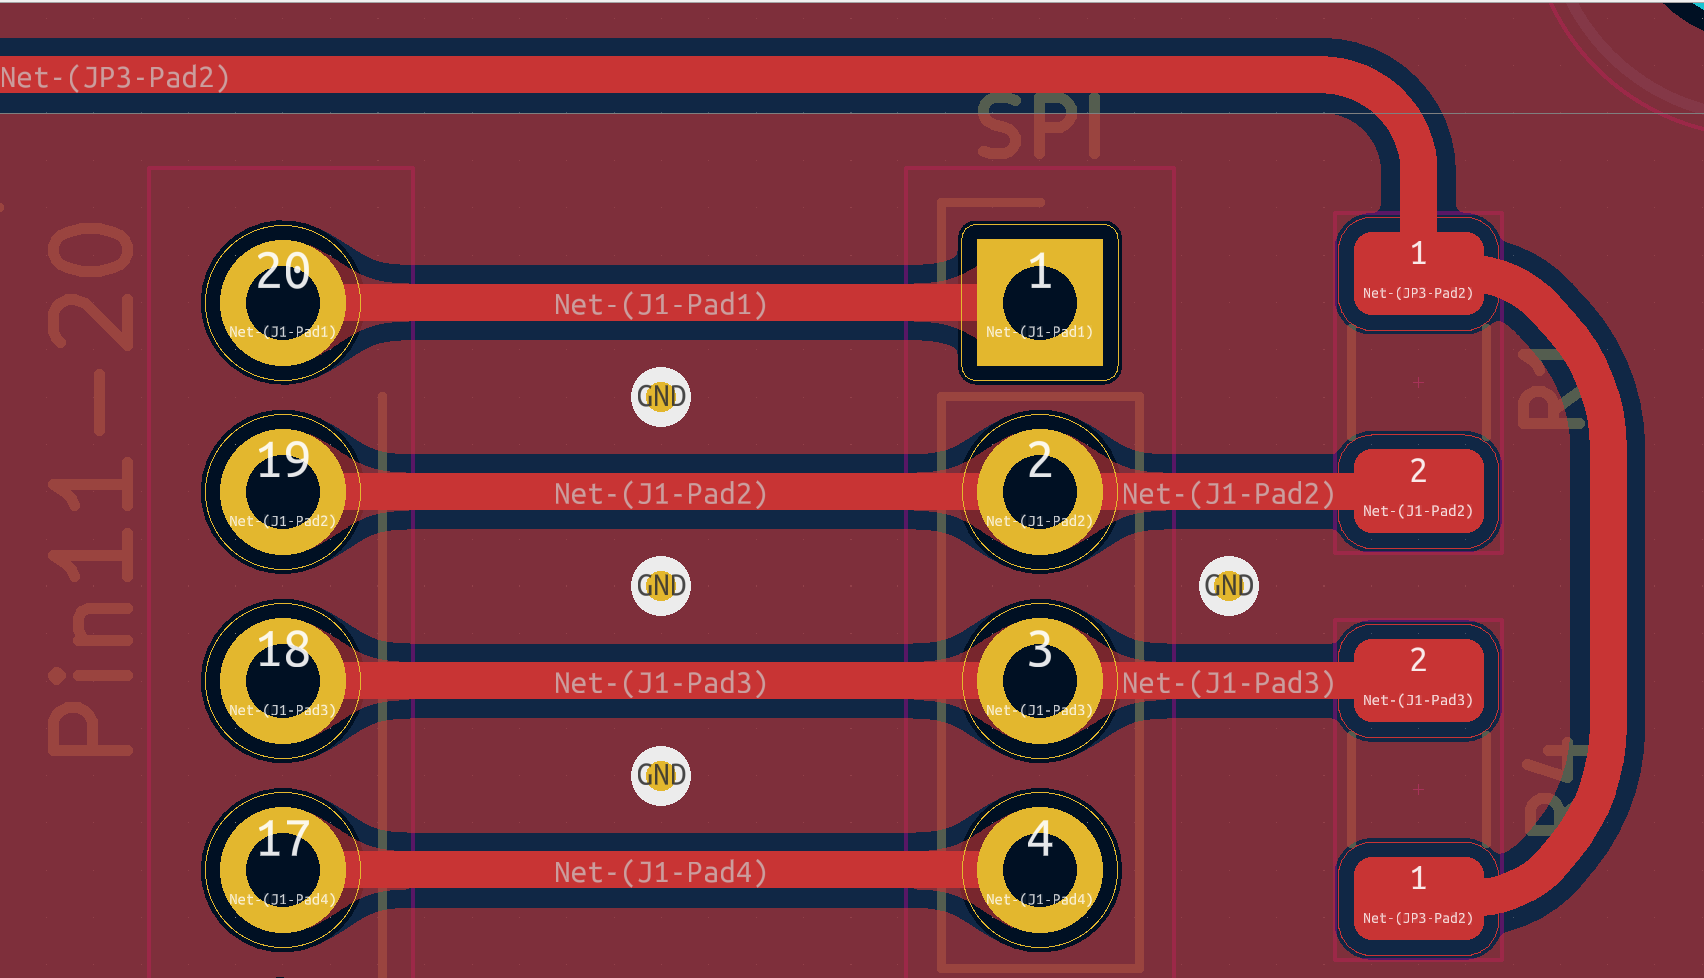
\includegraphics[trim=1mm 1mm 1mm 1mm,scale=0.33]{spi kimenet.PNG}
	\caption{SPI kimenet}
	\label{SPI kimenet}
\end{figure}
Kissé túl van tervezve az SPI csatlakozó, hiszen nem óriási frekvenciákon használom. De a túl tervezés ebben az esetben nem árt. A chip select, MISO, MOSI, és CLK vonalak mind ugyan olyan hosszúak. Ezt „length matching” nek hívjuk. Akkor fontos, ha akkora az adatátviteli alap frekvencia, hogy két vonal hossz különbségéből származó kettő közötti fázistolás gondot okoz a mintavételezésnél. A vonalak egymástól GND-vel le vannak árnyékolva, ez segíti, hogy a vonalak elektromágneses zaja kevésbé befolyásolják egymást.
\subsubsection{Az I2C csatlakozó}
\begin{figure}[H]
	\centering
	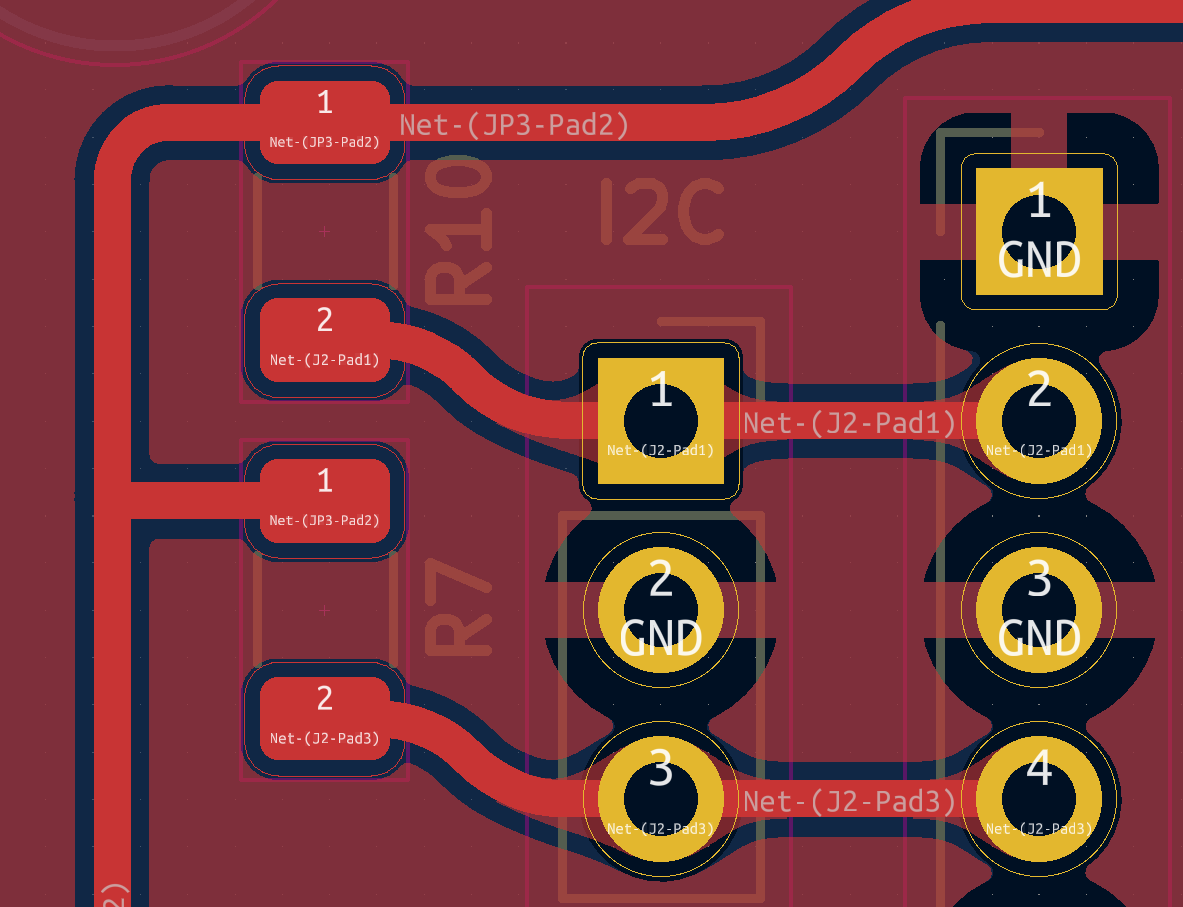
\includegraphics[trim=1mm 1mm 1mm 1mm,scale=0.45]{i2ckimenet.PNG}
	\caption{I2C kimenet}
	\label{I2C kimenet}
\end{figure}
Itt is inkább túl terveztem a kimenetet, mint alul. Itt is a SCL IS SDA vonal „length match”-elve van. Illetve az árnyékolást még a csatlakozókra is kiterjed. Így egészen a FPGA pin-ekhez az árnyékolást végig lehet vinni ha a SCL és SCL-hez tartozó lábak közötti lábat logikai ’0’-ra alítom.
\subsubsection{Plugin-ek}
Én két plug-in-t használtam. Az egyik a rounded tracks plug-in. Ami igazából csak esztétikai változásokat kreál a nyákon.
A plugin-t nagyon egyszerű használni. A következő kép a UI-ja.
\begin{figure}[H]
	\centering
	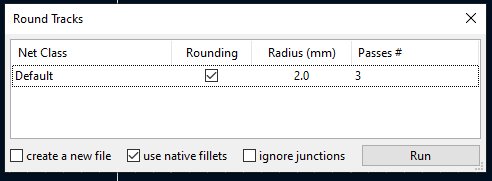
\includegraphics[trim=1mm 1mm 1mm 1mm,scale=0.75]{rounded ui.PNG}
	\caption{A rounded tracks plugin UI-ja}
	\label{A rounded tracks plugin UI-ja}
\end{figure}
A UI egyszerű. Netlista ként ki lehet választani, hogy kerekítse a plugin a netlistához tartozó trace-eket vagy nem. Ki lehet választani célzott rádiuszt, illetve,  hogy hányszor fusson a programm. A Run gombbal kell elindítani.

Ezek pedig arról képek hogy hogyan néz ki egy trace a plugin használata előtt és utána
Előtte:
\begin{figure}[H]
	\centering
	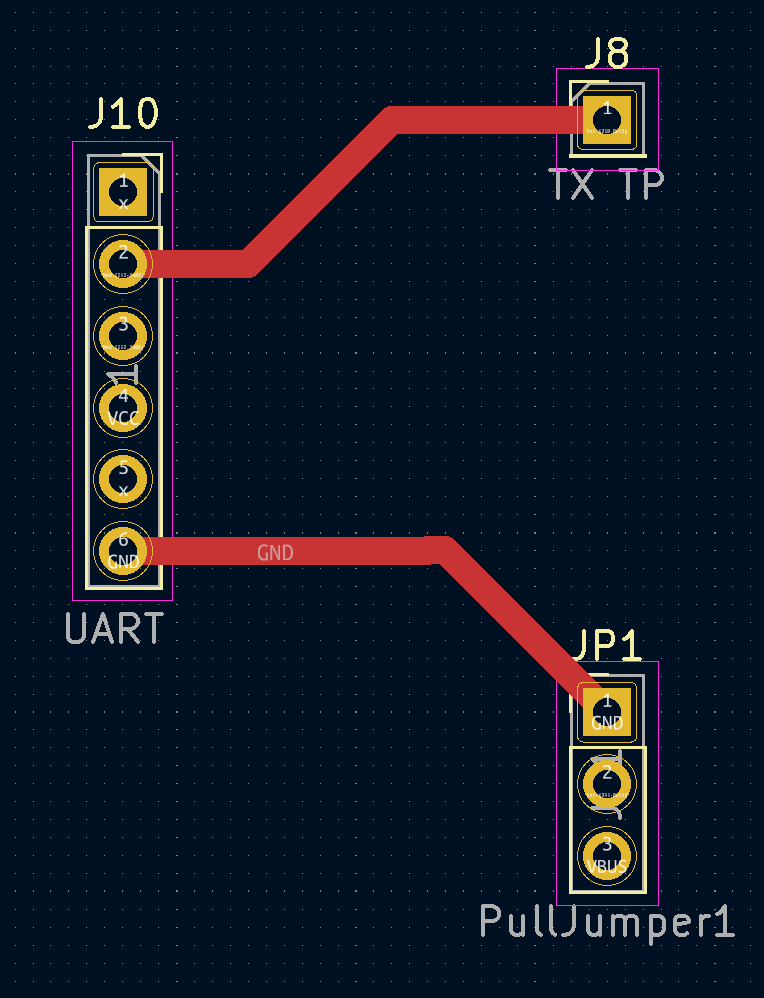
\includegraphics[trim=1mm 1mm 1mm 1mm,scale=0.35]{beforrounded.PNG}
	\caption{Egy trace a plugin használata előtt}
	\label{Egy trace a plugin használata előtt}
\end{figure}
\begin{figure}[H]
	\centering
	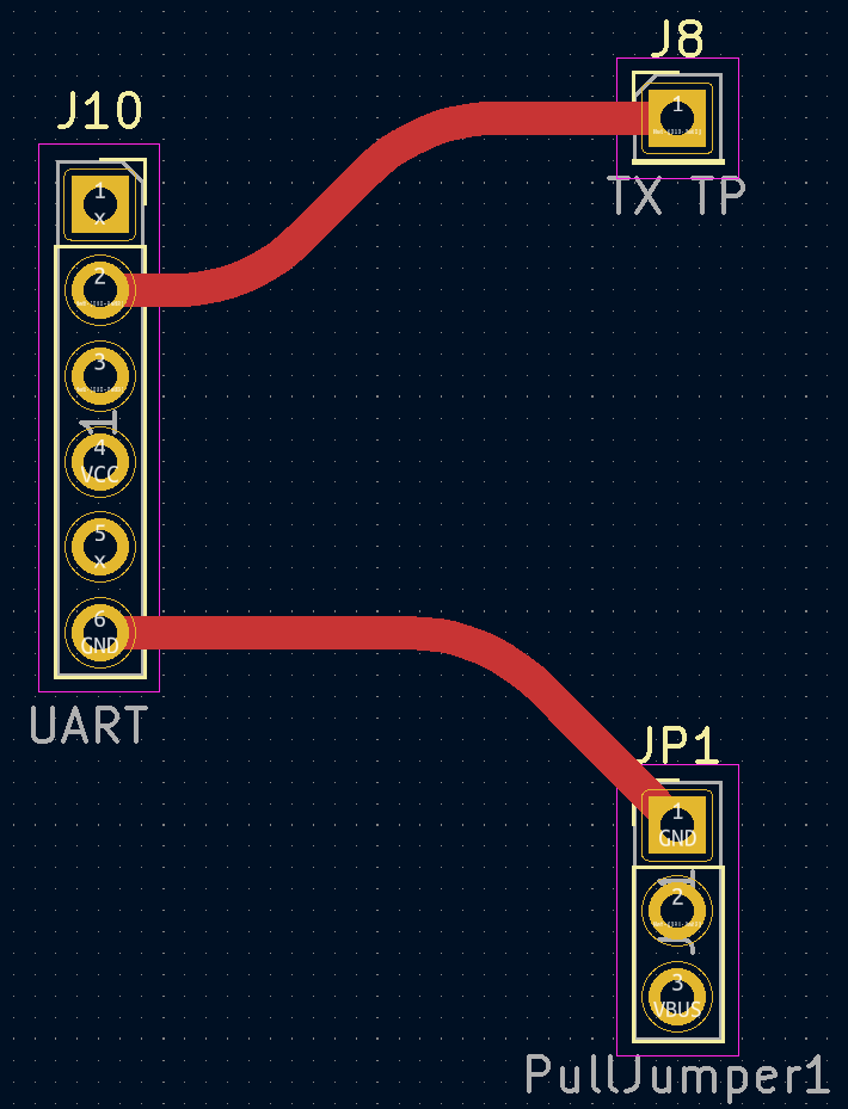
\includegraphics[trim=1mm 1mm 1mm 1mm,scale=0.35]{afterrounded.PNG}
	\caption{Egy trace a plugin használata után}
	\label{Egy trace a plugin használata után}
\end{figure}
Fontos hogy a plugin használata előtt nézzük át a tarce-einket. A plugin nem működik jól, ha túl sok elemre bontott csúnyán tervezett trace-et akarunk kerekíteni.
\begin{figure}[H]
	\centering
	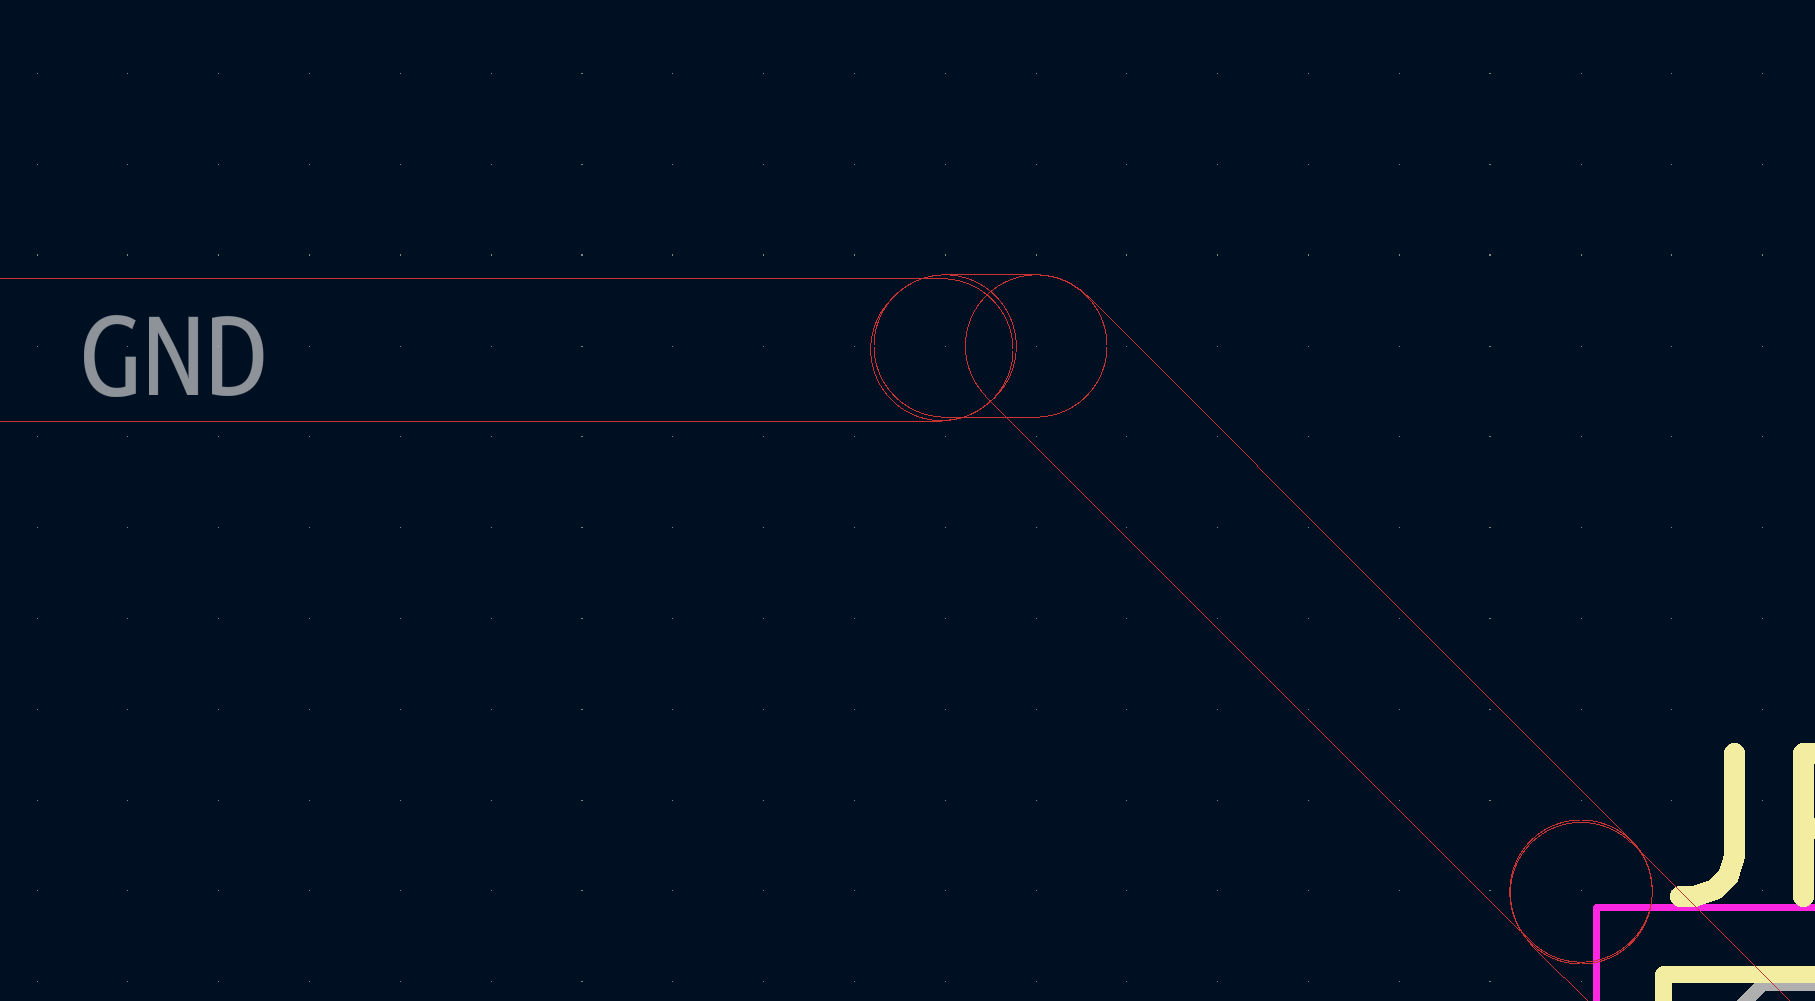
\includegraphics[trim=1mm 1mm 1mm 1mm,scale=0.25]{rosszpelda.PNG}
	\caption{Példa egy csúnyán tervezett trace-re}
	\label{Példa egy csúnyán tervezett trace-re}
\end{figure}
A másik plug-in pedig a Teardrop vias plug in. Ez is egy egyszerű plug-in ami részben Esztétikailag szépíti a nyák tervet, de fontos, hogy az éles sarkokat minimalizálja is. Hiszen az éles sarkok savcsapdákat okozhatnak, ahol a maratáshoz használt savak egy része megmarad, és az éles sarkoknál tovább korrodálja a rezet. A következő kép a UI-ja.
\begin{figure}[H]
	\centering
	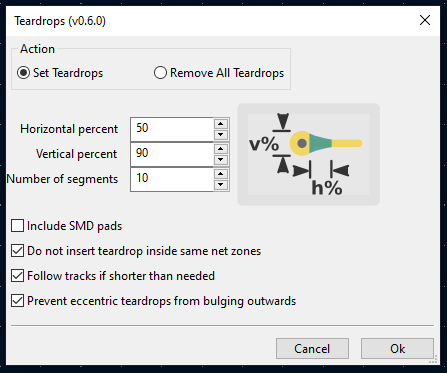
\includegraphics[trim=1mm 1mm 1mm 1mm,scale=0.75]{rounded vias ui.PNG}
	\caption{Teardrop vias UI} 
	\label{Teardrop vias UI}
\end{figure}
Ez pedig arról kép hogy hogyan néz ki egy via a plugin használata előtt és utána.
\begin{figure}[H]
	\centering
	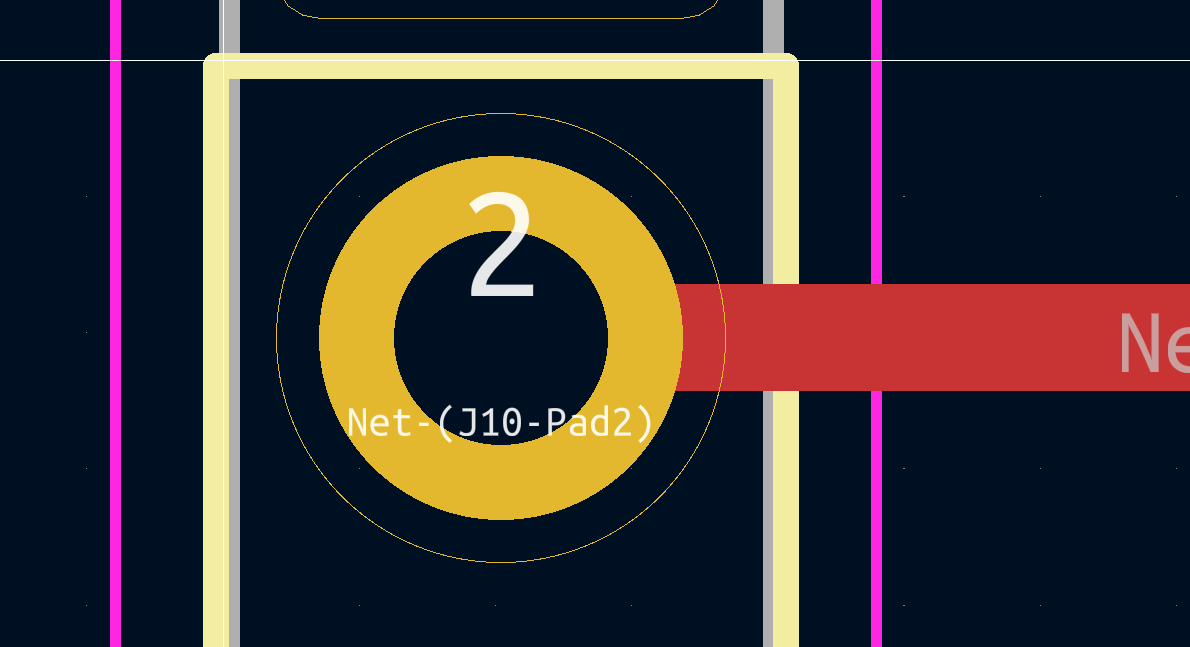
\includegraphics[trim=1mm 1mm 1mm 1mm,scale=0.4]{viabefore.PNG}
	\caption{Teardrop plugin használata előtt}
	\label{Teardrop plugin használata előtt} 
\end{figure}
\begin{figure}[H]
	\centering
	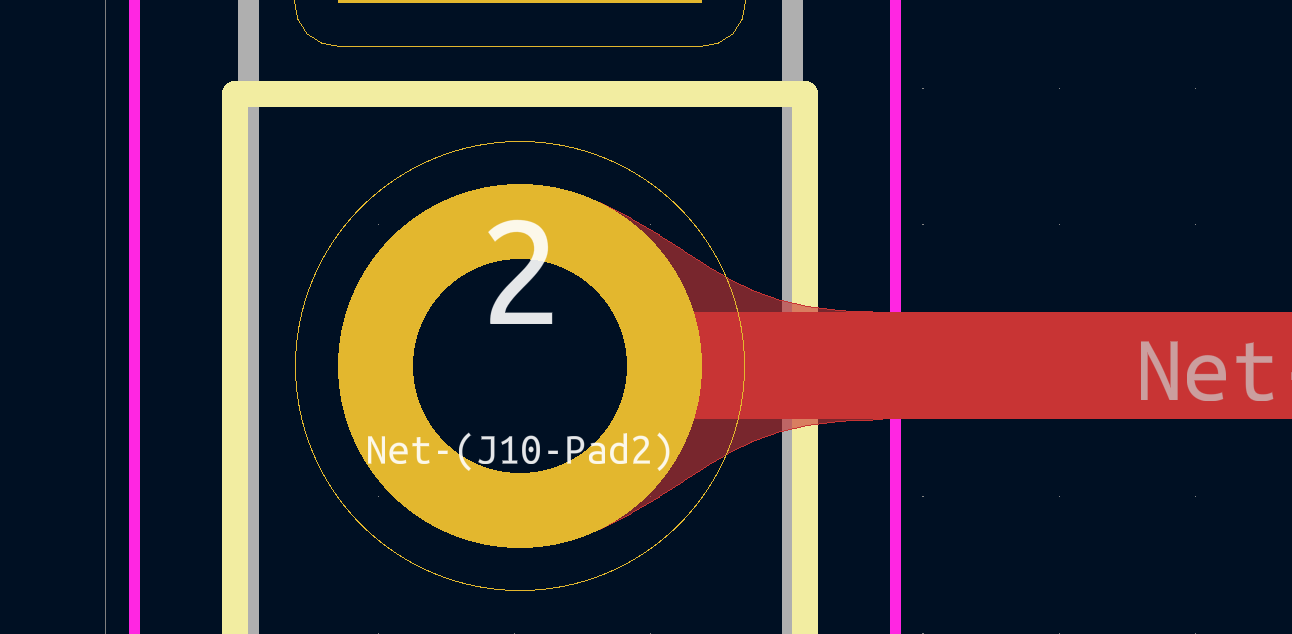
\includegraphics[trim=1mm 1mm 1mm 1mm,scale=0.4]{viaafter.PNG}
	\caption{Teardrop plugin használata után}
	\label{Teardrop plugin használata után} 
\end{figure}
\section{A Kész NYÁK}
\begin{figure}[H]
	\centering
	\includegraphics[trim=1mm 1mm 1mm 1mm,scale=0.125]{PCB.png}
	\caption{A Kész NYÁK}
	\label{A kész NYÁK} 
\end{figure}
\begin{figure}[H]
	\centering
	\includegraphics[trim=1mm 1mm 1mm 1mm,scale=0.125]{PCBassembled.png}
	\caption{A kész NYÁK összerakva és forrasztva}
	\label{A kész NYÁK összerakva és forrasztva} 
\end{figure}

\section{A Programozó al-entitásai}
A következőkben bemutatom az al-entitásokat, amiket használtam a programozóban. Mindet én terveztem és írtam meg, kivéve az Int\_Osc entitást, amit az FPGA-m gyártója által adott módon írtam meg.
\subsection{A Int\_Osc entitás}
Az Int\_Osc egy belső oszcillátor modult valósít meg, amely egy órajelet generál a rendszer számára. Ez a modul a MachXO2 FPGA belső oszcillátorát használja, amely egy konfigurálható frekvenciájú órajelet biztosít. 


Az Int\_Osc entitás két portot tartalmaz:
\begin{itemize}
	\item StdBy (in std\_logic): Ez a bemeneti jel az oszcillátor készenléti (standby) állapotát vezérli. Ha a jel aktív, az oszcillátor leáll, és nem generál órajelet. Ha inaktív, az oszcillátor működik és órajelet generál.
	\item Clk (out std\_logic): Ez a kimeneti jel az oszcillátor által generált órajelet biztosítja a rendszer többi részének.
\end{itemize}

Az architektúra az FPGA belső oszcillátorát (OSCH komponens) használja. Az OSCH komponens a következőket tartalmazza:

\begin{itemize}
	\item NOM\_FREQ (generikus paraméter): Az oszcillátor névleges frekvenciáját határozza meg. Az alapértelmezett érték itt "9.17", ami 9,17 MHz-es órajelet jelent.
	\item STDBY (bemenet): Az oszcillátor készenléti állapotát vezérli.
	\item OSC (kimenet): Az oszcillátor által generált órajel.
	\item SEDSTDBY (kimenet): Egy diagnosztikai jel, amely az oszcillátor készenléti állapotát jelzi (ebben az implementációban nem használják).
\end{itemize}

Az architektúra a következőképpen működik:

\begin{enumerate}
	\item Az OSCH komponens egy példányát (OSCInst0) hozza létre.
	\item A NOM\_FREQ generikus paraméter értéke "9.17", amely meghatározza az oszcillátor frekvenciáját. Ez választhatóan módosítható a tervező által.
	\item A STDBY bemenet az Int\_Osc entitás StdBy portjához van kötve.
	\item Az OSC kimenet az Int\_Osc entitás Clk portjához van kötve.
\end{enumerate}

Az Int\_Osc modul a rendszer órajelének biztosítására szolgál. Az óra jelet a rendszer összes része használja a szinkron működéshez.

\subsubsection{Az órajel sebeségének válastása}
A FPGA belő órajel sebességét  adott értékekből lehet választani. Az FPGA termékcsalád adatlapja szerint ezek a sebességek közül lehet:
\begin{figure}[H]
	\centering
	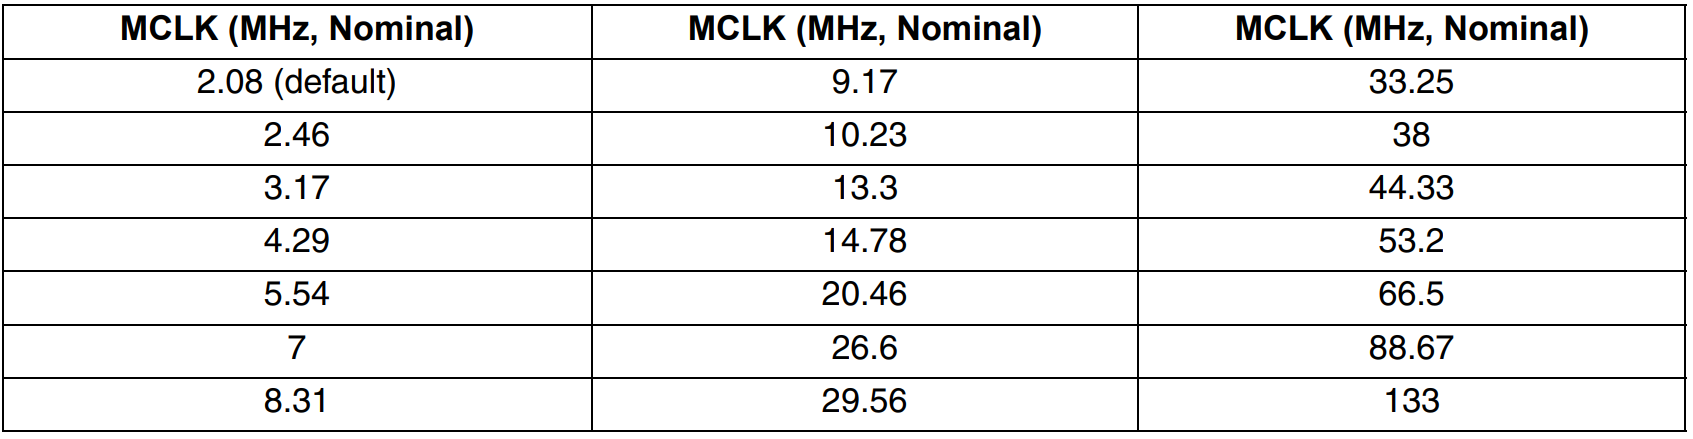
\includegraphics[trim=1mm 1mm 1mm 1mm,scale=0.344]{clkrates.PNG}
	\caption{Elérhető CLK-frekvenciák az FPGA adatlapja alapján \cite{fpgaadatlap}}
	\label{Elérhető CLK-frekvenciák az FPGA adatlapja alapján } 
\end{figure}
Az óra jelet úgy kell választani, hogy elég gyors legyen, hogy a design megoldja a feladatot amire tervezve lett. Gyorsabbra nem érdemes, mert az felesleges slack problémákhoz vezethet. 

A programozóban az órajelnek legalább 4-szer gyorsabbnak kell lennije, mint a célzott I2C órajel sebessége, mert az I2C órajelenként 4 műveletet végzik a I2C entitás. És 2 szer gyorsabbnak, mint a célzott SPI órajel, mert az SPI órajelenként 2 műveletet végzik a SPI entitás.
Az én célzott I2C órajelsebességem nagyobb mint a célzott uart baud ráta de lassab mint  1MHz-nel. Ez azért van, mert a legtöbb modern EEPROM képes 1MHz órajelsebességre, és ki szeretném használni ezt a sebességet. És azert kell hogy gyorsabb legyen az I2C mint az UART mert az I2C tud "várni" az UART adatra órajelnyújtással, de a UART nem tud "várni" a I2C-re mert az UART aszinkron. Az SPI célsebesség pedig 5MHz körül van, hasonló okok miatt.

A programozóm UART-ot is használ,  amint előbb volt tárgyalva, egy aszinkron kommunikációs protokoll. Ez azt jelenti, hogy a belső óra jelet úgy kell választani, hogy jól leosztható legyen a megcélzott baud rátához. Tegyük fel, hogy  a célzott baud ráta 23040. Ha a  belső órajel 2.46MHz akkor az órajelosztó számlálónak 11-ig kell számolnia, mivel \(230400$baud$ / 2.46$MHz $ = 10.68\). Egy órajel számláló csak egész számokkal tud számolni. így minden egyes periódus alatt fél óra jelet késne a belső UART számlálá a tényleges 230400 baud-hoz. Úgy kellet választanom az óra jelet, hogy minimális kerekítéssel  le lehessen osztania és ez a késés minimális legyen. A célzott AURT sebesség 576000 baud.

Ezek miatt választottam a 9.17MHz-t belső órajelnek. Így a UART osztó hiba 0.08 órajel per baud periódus. A I2C maximum sebessége 2.29MHz. Az SPI Max sebessége 4.59MHz.

\subsection{A write8bit entitás}
A write8bit e8 bites adat írására szolgál az SPI vonalokon. Az entitás bemeneti és kimeneti portjai a következők:

Portok:
\begin{itemize}
	\item iCS: Bemeneti vezérlőjel, amely az írási folyamat indítását jelzi ('0' értékkel aktiválódik).
	\item cs: Kimeneti vezérlőjel, amely az írási folyamat állapotát jelzi ('1' az alapértelmezett érték).
	\item Clk: Órajel bemenet, amely az állapotgép működését vezérli.
	\item Done: Kimeneti jel, amely az írási folyamat befejezését jelzi ('1' az alapértelmezett érték).
	\item bit8SCL: Órajel kimenet a soros kommunikációhoz ('1' az alapértelmezett érték).
	\item nReset: Reset bemenet, amely az állapotgépet alaphelyzetbe állítja ('0' értékkel aktiválódik).
	\item bit8SDA: Adat kimenet a soros kommunikációhoz ('1' az alapértelmezett érték).
	\item SDA\_data: 8 bites adat bemenet, amelyet a modul sorosan továbbít.
\end{itemize}
A write8bit entitás egy állapotgépet tartalmaz, amely három állapotból áll:
\begin{enumerate}
	\item Idle: Alapértelmezett állapot, ahol az órajel (bit8SCL) és az adatvonal (bit8SDA) magas szinten van, és a Done jel aktív ('1'). Ha az iCS bemenet alacsony szintre kerül ('0'), az állapotgép a write8 állapotba lép.
	\item write8: Az adat írásának állapota. Az adatot a SDA\_data bemenetről bitenként továbbítja a bit8SDA kimenetre. Az írási folyamatot a BitIndex számláló vezérli, amely 0-tól 7-ig számol. Ha az összes bitet elküldte, az állapotgép a stop állapotba lép.
	\item stop: Az írási folyamat lezárása. A cs jel visszaáll magas szintre ('1'), és az állapotgép visszatér az Idle állapotba.
\end{enumerate}
Az állapotgép működését az órajel (Clk) vezérli, és az nReset bemenet bármikor alaphelyzetbe állíthatja. A Main entitásban ez az entitás felelős az egyszerű csupán 8bites egyirányú (MOSI) SPI kommunikációkért. 
\subsection{UART\_TX entitás}
A UART\_TX az UART protokoll szerinti adatküldést valósítja meg. Ez a modul soros adatátvitelre szolgál, ahol a bemeneti adatokat bitenként továbbítja egy kimeneti vonalon

Portok:
\begin{itemize}
	\item TXData: 8 bites bemeneti adat, amelyet a modul sorosan továbbít.
	\item Clk: Órajel bemenet, amely az állapotgép működését vezérli.
	\item SendTX: Bemeneti vezérlőjel, amely az adatküldés indítását jelzi ('1' értékkel aktiválódik).
	\item TXDone: Kimeneti jel, amely az adatküldés befejezését jelzi ('1' az alapértelmezett érték).
	\item nReset: Reset bemenet, amely az állapotgépet alaphelyzetbe állítja ('0' értékkel aktiválódik).
	\item TXOut: Kimeneti adatvonal, amelyen a soros adatátvitel történik.
	\item TXActive: Kimeneti jel, amely az adatküldés aktív állapotát jelzi ('1', ha a modul éppen adatot küld).
\end{itemize}
Generikus paraméter:
\begin{itemize}
	\item ClkRatio: Az órajel osztására szolgáló paraméter, amely meghatározza az UART adatátviteli sebességét (baud rate).
\end{itemize}
A UART\_TX entitás egy állapotgépet tartalmaz, amely az UART adatküldési folyamatát valósítja meg. Az állapotgép az alábbi állapotokból áll:
\begin{enumerate}
	\item Idle: Alapértelmezett állapot, ahol a modul várakozik a SendTX jel aktiválására. Az órajel számláló (ClkCount) nullázódik, és a kimeneti vonal (TXOut) magas szinten van ('1').
	\item StartBit: Az adatküldés kezdő bitje ('0') kerül a kimeneti vonalra. Az órajel számláló növekszik, és ha eléri a ClkRatio értéket, az állapotgép a DataBits állapotba lép.
	\item DataBits: Az adatbitek soros továbbítása történik. A TXData bemenet bitjeit a BitIndex számláló segítségével küldi ki a modul. Ha az összes bit elküldésre került, az állapotgép a StopBit állapotba lép.
	\item StopBit: Az adatküldés záró bitje ('1') kerül a kimeneti vonalra. Az órajel számláló növekszik, és ha eléri a ClkRatio értéket, az állapotgép a FrameEnd állapotba lép.
	\item FrameEnd: Az adatküldés befejeződik, a TXActive jel inaktívvá válik ('0'), és a TXDone jel aktívvá válik ('1'). Az állapotgép visszatér az Idle állapotba.
\end{enumerate}
Az állapotgép működését az órajel (Clk) vezérli, és az nReset bemenet bármikor alaphelyzetbe állíthatja.

\subsection{A UART\_RX entitás}
A UART\_RX entitás a protokoll szerinti adatfogadást valósítja meg. Ez a modul soros adatokat fogad egy bemeneti vonalon, és azokat párhuzamos formátumba alakítja.
\begin{itemize}
	\item Clk: Órajel bemenet, amely az állapotgép működését vezérli.
	\item RXIn: Soros adat bemenet, amelyen keresztül az UART adatokat fogadja.
	\item Ack: Bemeneti vezérlőjel, amely az adatfogadás befejezésének visszaigazolására szolgál.
	\item RXData: 8 bites kimeneti adat, amely a fogadott adatot tartalmazza.
	\item RXDataReady: Kimeneti jel, amely az adatfogadás befejezését jelzi ('1' értékkel aktiválódik).
	\item nReset: Reset bemenet, amely az állapotgépet alaphelyzetbe állítja ('0' értékkel aktiválódik).
	\item RXActive: Kimeneti jel, amely az adatfogadás aktív állapotát jelzi.
\end{itemize}
Generikus paraméterek:
\begin{itemize}
	\item ClkRatio: Az órajel osztására szolgáló paraméter, amely meghatározza az UART adatátviteli sebességét (baud rate).
	\item CRHalf: Az órajel osztásának felezett értéke, amely a bitközép detektálására szolgál.
\end{itemize}
A UART\_RX entitás egy állapotgépet tartalmaz, amely az UART adatfogadási folyamatát valósítja meg. Az állapotgép az alábbi állapotokból áll:
\begin{enumerate}
	\item Idle: Alapértelmezett állapot, ahol a modul várakozik az adatfogadás kezdetére. Ha a RXIn jel alacsony szintre kerül ('0'), az állapotgép a StartBit állapotba lép.
	\item StartBit: Az adatfogadás kezdő bitjének ('0') detektálása történik. Az órajel számláló (ClkCount) növekszik, és ha eléri a ClkRatio értéket, az állapotgép a DataBits állapotba lép.
	\item DataBits: Az adatbitek fogadása történik. A RXIn bemenet bitjeit a SData regiszterbe menti a modul, a BitIndex számláló segítségével. Ha az összes bitet fogadta, az állapotgép a StopBit állapotba lép.
	\item StopBit: Az adatfogadás záró bitjének ('1') detektálása történik. A RXDataReady jel aktívvá válik ('1'), jelezve, hogy az adat fogadása befejeződött. Ha az Ack jel aktív ('1'), az állapotgép visszatér az Idle állapotba.
\end{enumerate}
Az állapotgép működését az órajel (Clk) vezérli, és az nReset bemenet bármikor alaphelyzetbe állíthatja.
\subsection{A writePage entitás}
A writePage entitás a komplexebb SPI kommunikációkat kezeli. A neve writepage maradt, mert eredetileg a tervem az volt, hogy két entitást csinálok. Egy entitást, ami az SPI írásért felelős, egy pedig ami az olvasásért felelős. De végül egyszerűbb volt egy entitásban megvalósítani mind két funkciót.
Ez az entitás azért is komplexebb mert, eltérően a write8bi-től képes a kommunikációs protokoll kerete hosszán alítani.

Portok:
\begin{itemize}
	\item iCS: Bemeneti vezérlőjel, amely az adatátviteli folyamat indítását jelzi ('0' értékkel aktiválódik).
	\item RW: Bemeneti jel, amely az írási ('0') vagy olvasási ('1') műveletet határozza meg.
	\item Rdy: Kimeneti jel, amely az adatátviteli folyamat készenlétét jelzi ('1' az alapértelmezett érték).
	\item cs: Kimeneti vezérlőjel, amely az adatátvitel állapotát jelzi ('1' az alapértelmezett érték).
	\item from\_SDO: Bemeneti adatvonal, amelyen keresztül az olvasott adat érkezik.
	\item Done: Kimeneti jel, amely az adatátviteli folyamat befejezését jelzi ('1' az alapértelmezett érték).
	\item toSCL: Órajel kimenet a soros kommunikációhoz ('1' az alapértelmezett érték).
	\item nReset: Reset bemenet, amely az állapotgépet alaphelyzetbe állítja ('0' értékkel aktiválódik).
	\item toSDA: Adat kimenet a soros kommunikációhoz ('1' az alapértelmezett érték).
	\item MISO\_DR: Kimeneti jel, amely az olvasási művelet befejezését jelzi.
	\item next8bits: 8 bites bemeneti adat, amelyet a modul írni fog.
	\item read8bits: 8 bites kimeneti adat, amely az olvasott adatot tartalmazza.
	\item RW\_length: Az SPI művelet teljes hosszát meghatározó bemeneti paraméter (bájtokban).
	\item RH\_length: Az olvasási művelet címző keret hosszát meghatározó bemeneti paraméter (bájtokban).
\end{itemize}
Az állapotgép működését az órajel (Clk) vezérli, és az nReset bemenet bármikor alaphelyzetbe állíthatja.
Az állapotgép négy fő állapotot tartalmaz:

\begin{enumerate}
	\item Idle (Alapállapot) \begin{itemize}
		\item Funkció: Az állapotgép várakozik, amíg az iCS jel alacsony szintre kerül ('0'), ami az SPI kommunikáció kezdetét jelzi.
		\item Tevékenységek: \begin{itemize}
			\item Az összes kimeneti jel alaphelyzetbe állítása.
			\item Az RW jel értéke a RWlatch jelbe kerül.
			\item Ha iCS = '0', akkor: \begin{itemize}
				\item Az állapot write8-ra vált
				\item cs = '0' (chip select aktív).
				\item Done = '0' (művelet folyamatban).
				\item A next8bits bemeneti adatot a current8bits jel tárolja.
			\end{itemize}
		\end{itemize}
	\end{itemize}
	\item write8 (Írási állapot) \begin{itemize}
		\item Funkció: Az aktuális 8 bites adat (current8bits) bitenként kerül kiküldésre az SPI buszra.
		\item Tevékenységek: \begin{itemize}
			\item Az toSDA jel az aktuális bit értékét veszi fel (current8bits(7-BitIndex)).
			\item Az toSCL jel váltakozik ('0' → '1'), hogy az órajelet biztosítsa.
			\item A BitIndex növekszik minden bit kiküldése után.
			\item Ha az összes bit kiküldésre került (BitIndex = 7), akkor: \begin{itemize}
				\item Az állapot stop-ra vált.
				\item A BitIndex alaphelyzetbe áll.
			\end{itemize}
		\end{itemize}
	\end{itemize}
	\item read8 (Olvasási állapot) \begin{itemize}
		\item Funkció: Az SPI buszról érkező adatot bitenként olvassa be.
		\item Tevékenységek: \begin{itemize}
			\item Az toSCL jel váltakozik ('0' → '1'), hogy az órajelet biztosítsa.
			\item Az from\_SDO bemeneti jel értéke a read8bits jel megfelelő bitjébe kerül (read8bits(7-BitIndex)).
			\item A BitIndex növekszik minden bit beolvasása után.
			\item Ha az összes bit beolvasásra került (BitIndex = 7), akkor: \begin{itemize} 
			\item Az állapot stop-ra vált.
			\item A MISO\_DR jel '1'-re áll, jelezve, hogy az adat érvényes.
			\end{itemize}
		\end{itemize}
	\end{itemize}
	\item stop (Befejezési állapot) \begin{itemize}
		\item Itt történik az állapotok közötti váltási logika az iCS, RW, BitIndex, és ByteIndex jelek alapján. Mindig várja az iCS jel alacsony szintjét, mielőtt állapotot vált.  Ha a RWlatch = ’1’, akkor felelős annak ellenőrzéséért, hogy az SPI üzenet elérte-e a megadott fejléc hosszúságát. Ha igen, akkor write8 helyett read8-be ugrik. Illetve, ha az üzenet elérte a teljes hosszát, visszatér az Idle állapotba.
	\end{itemize}
\end{enumerate}
\subsection{A I2C entitás}
Az I2C entitás az IC2 protokoll szerinti adatátvitelt valósítja meg. Ez az entitás képes adatokat írni és olvasni egy I2C buszon, és támogatja a protokollhoz szükséges vezérlőjelek generálását. Ez az entitás is komplex, képes írni/olvasni és a kommunikációs protokoll kerete hosszán alítani.

Portok:
\begin{itemize}
	\item DataIn: 8 bites bemeneti adat, amelyet a modul az I2C buszra ír.
	\item DataOut: 8 bites kimeneti adat, amely az I2C buszról olvasott adatot tartalmazza.
	\item RW\_length: Az írási művelet hosszát meghatározó bemeneti paraméter (bájtokban).
	\item RH\_length: Az olvasási művelet címző keret hosszát meghatározó bemeneti paraméter (bájtokban).
	\item Clk: Órajel bemenet, amely az állapotgép működését vezérli.
	\item Go: Bemeneti vezérlőjel, amely az I2C művelet indítását jelzi.
	\item Send\_i2c: Bemeneti jel, amely az I2C adatátvitel indítását szabályozza.
	\item nReset: Aszinkron reset bemenet, amely az állapotgépet alaphelyzetbe állítja ('0' értékkel aktiválódik).
	\item RW: Bemeneti jel, amely az írási ('0') vagy olvasási ('1') műveletet határozza meg.
	\item rSDA: Kétirányú adatvonal az I2C buszhoz.
	\item rSCL: Órajel kimenet az I2C buszhoz.
	\item dataready: Kimeneti jel, amely az adatátvitel befejezését jelzi.
	\item atstop: Kimeneti jel, amely az I2C stop feltétel elérését jelzi.
	\item Done: Kimeneti jel, amely az I2C művelet befejezését jelzi.
\end{itemize}
A célzott órajelsebesség mint előbb említettem 576kHz és 1MHz között van. A belső órajel 9.17MHz, így 15-tel leosztva az I2C órajel 661kHz.

Állapotok Leírása:
\begin{itemize}
	\item off \begin{itemize}
		\item Cél: Ez az alapértelmezett, nyugalmi állapot, ahol az I2C modul várakozik az indító jelre.
		\item Műveletek: Az összes belső számláló (Bitcount, Bytecount, count) és retesz (RWlatch,dataready) alaphelyzetbe állítása.
		\item Átmenet: Send\_i2c = '1' esetén az állapot start-ra vált.
	\end{itemize}
	\item start \begin{itemize}
		\item Cél: Az I2C start feltétel generálása.
		\item Műveletek: \begin{itemize}
			\item A SDAen és SCLen jelek váltogatása a start feltétel létrehozásához.
			\item A count jel növelése az időzítés nyomon követésére.
		\end{itemize}
		\item Átmenet: 15 órajelciklus után az állapot PFHW-ra vált.
	\end{itemize}

	 \item PFHW (Packet Frame Header and Write):
    \begin{itemize}
        \item Cél: Az adatcsomag fejlécének és az adatok bitenkénti továbbítása.
        \item Műveletek:
        \begin{itemize}
            \item A SDAen jel meghajtása a DataIn aktuális bitjével.
            \item A SCLen váltogatása órajelek generálásához.
            \item A bit- és bájtszámlálók (Bitcount, Bytecount) nyomon követése.
        \end{itemize}
        \item Átmenet:
        \begin{itemize}
            \item 8 bit (1 bájt) továbbítása után az állapot wack-ra vált.
            \item Több bájt esetén a Bytecount növekszik.
        \end{itemize}
    \end{itemize}
    \item wack (Write Acknowledge):
    \begin{itemize}
        \item Cél: Az írási művelet után a slave eszköz visszaigazolásának (ACK) várakozása.
        \item Műveletek:
        \begin{itemize}
            \item A SDAen jel '1' értékre állítása az SDA vonal felszabadításához.
            \item A SCLen váltogatása órajelek generálásához.
            \item A golatch jel ellenőrzése a következő művelet meghatározásához.
        \end{itemize}
        \item Átmenet:
        \begin{itemize}
            \item Ha golatch = '1', az állapot PFHW-ra vált további adatátvitelhez.
            \item Ha az írási művelet befejeződött (Bytecount = RW\_length), az állapot stop-ra vált.
            \item Ha olvasási műveletre váltás történik (Bytecount >= RH\_length), az állapot readB-re vált.
        \end{itemize}
    \end{itemize}
    \item readB (Read Byte):
    \begin{itemize}
        \item Cél: Egy bájt adat olvasása a slave eszközről.
        \item Műveletek:
        \begin{itemize}
            \item A SDAen jel '1' értékre állítása az SDA vonal felszabadításához.
            \item Az rSDA értékének rögzítése a DataOut jelbe a 8. órajelciklus alatt.
            \item A SCLen váltogatása órajelek generálásához.
            \item A bit- és bájtszámlálók (Bitcount, Bytecount) nyomon követése.
        \end{itemize}
        \item Átmenet:
        \begin{itemize}
            \item 8 bit (1 bájt) olvasása után az állapot rack-ra vált.
        \end{itemize}
    \end{itemize}
    \item rack (Read Acknowledge):
    \begin{itemize}
        \item Cél: Visszaigazolás (ACK) küldése a slave eszköznek az olvasási művelet után.
        \item Műveletek:
        \begin{itemize}
            \item A SDAen jel '0' értékre állítása ACK küldéséhez, vagy '1' értékre NACK küldéséhez (ha az olvasási művelet befejeződött).
            \item A SCLen váltogatása órajelek generálásához.
            \item A golatch jel ellenőrzése a következő művelet meghatározásához.
        \end{itemize}
        \item Átmenet:
        \begin{itemize}
            \item Ha golatch = '1', az állapot readB-re vált további adatfogadáshoz.
            \item Ha az olvasási művelet befejeződött (Bytecount = RW\_length), az állapot stop-ra vált.
        \end{itemize}
    \end{itemize}
    \item restart:
    \begin{itemize}
        \item Cél: Ismételt start feltétel generálása több részből álló tranzakciókhoz.
        \item Műveletek:
        \begin{itemize}
            \item A SDAen és SCLen váltogatása az ismételt start feltétel létrehozásához.
            \item A count jel alaphelyzetbe állítása.
        \end{itemize}
        \item Átmenet: 15 órajelciklus után az állapot PFHW-ra vált.
    \end{itemize}
    \item stop:
    \begin{itemize}
        \item Cél: Az I2C stop feltétel generálása a kommunikáció befejezéséhez.
        \item Műveletek:
        \begin{itemize}
            \item A SDAen és SCLen váltogatása a stop feltétel létrehozásához.
            \item Az összes belső számláló (count, Bytecount) alaphelyzetbe állítása.
            \item A dataready jel '0' értékre állítása.
        \end{itemize}
        \item Átmenet: 15 órajelciklus után az állapot off-ra vált.
    \end{itemize}

\end{itemize}
\section{A fő (MAIN) entitás}
A main entitás biztosítja a programozó funkcionalitását, az összes alentitást használva. A felhasználó által küldött utasításokat értelmezi, és az USB-n keresztül küldött adatfolyamot továbbítja a I2C és SPI alentitásoknak. Azért is felelős, hogy a I2C és SPI adatfolyamok szinkronizálva maradjanak az UART adatfolyamatok. 
\subsection{A main entity állapotgépe}
\begin{itemize}
    \item 000 (Base State):
    \begin{itemize}
        \item Cél: Az alapállapot, ahol a rendszer várakozik a bemeneti jelekre.
        \item Műveletek:
        \begin{itemize}
            \item Az összes vezérlőjel alaphelyzetbe állítása.
            \item Ha az UART fogadási művelet befejeződött, az állapot a StateHolder értékére vált.
        \end{itemize}
        \item Átmenet: Az UART fogadási művelet (RXDR) és az SPI írási művelet (DoneW) befejeződése után.
    \end{itemize}
    \item 001 (SPI Configure):
    \begin{itemize}
        \item Cél: Egy bájtos SPI kommunikációk végrehajtása.
        \item Műveletek:
        \begin{itemize}
            \item Az SPI vonalak vezérlése a write8bit modul segítségével.
            \item Az UART fogadási adatainak (DataFromRx) továbbítása az SPI modul felé.
        \end{itemize}
        \item Átmenet: Az SPI művelet befejezése után visszatérés az alapállapotba.
    \end{itemize}
    \item 010 (SPI Read):
    \begin{itemize}
        \item Cél: Az SPI olvasási művelet végrehajtása.
        \item Műveletek:
        \begin{itemize}
            \item Az SPI olvasási művelet indítása a writePage modul segítségével.
            \item Az olvasott adat (SDO\_datap) továbbítása az UART felé.
        \end{itemize}
        \item Átmenet: Az SPI olvasási művelet befejezése után visszatérés az alapállapotba.
    \end{itemize}
    \item 011 (SPI Write):
    \begin{itemize}
        \item Cél: Az SPI írási művelet végrehajtása.
        \item Műveletek:
        \begin{itemize}
            \item Az SPI írási művelet indítása a writePage modul segítségével.
            \item Az UART fogadási adatainak (DataFromRx) továbbítása az SPI modul felé.
        \end{itemize}
        \item Átmenet: Az SPI írási művelet befejezése után visszatérés az alapállapotba.
    \end{itemize}
    \item 100 (Get Settings):
    \begin{itemize}
        \item Cél: A rendszer konfigurációs beállításainak frissítése.
        \item Műveletek:
        \begin{itemize}
            \item Az UART fogadási adatainak (DataFromRx) tárolása a settings vektorban.
        \end{itemize}
        \item Átmenet: A settings vektor feltöltése után visszatérés az alapállapotba.
    \end{itemize}
    \item 101 (I2C Read):
    \begin{itemize}
        \item Cél: Az I2C olvasási művelet végrehajtása.
        \item Műveletek:
        \begin{itemize}
            \item Az I2C olvasási művelet indítása az I2C modul segítségével.
            \item Az olvasott adat (i2c\_DataOut) továbbítása az UART felé.
        \end{itemize}
        \item Átmenet: Az I2C olvasási művelet befejezése után visszatérés az alapállapotba.
    \end{itemize}
    \item 110 (I2C Write):
    \begin{itemize}
        \item Cél: Az I2C írási művelet végrehajtása.
        \item Műveletek:
        \begin{itemize}
            \item Az I2C írási művelet indítása az I2C modul segítségével.
            \item Az UART fogadási adatainak (DataFromRx) továbbítása az I2C modul felé.
        \end{itemize}
        \item Átmenet: Az I2C írási művelet befejezése után visszatérés az alapállapotba.
    \end{itemize}
\end{itemize}
\section{C++ ban megírt utasítás küldő program}
\subsection{A Terminal app program}
A program célja, hogy hexadecimális formátumban megadott adatokat küldjön a számítógéphez csatlakoztatott programozónak egy COM soros porton keresztül, majd fogadja és megjelenítse a programozótól visszakapott adatokat.
\subsubsection{A program működése}
\begin{enumerate}
	\item Soros port megnyitása és beállítása.
\begin{itemize}
	\item A program a CreateFile függvénnyel megnyitja a COM portot olvasásra és írásra.
	\item A SetupComm függvénnyel 1 MB-os bemeneti és kimeneti puffert állít be a soros porthoz.
	\item A DCB struktúrában beállítja a kommunikációs paramétereket. Például: Baud rate: 576000, 8 adatbit, 1 stopbit, és paritás bit nélküli adatkeret.
	\item A COMMTIMEOUTS struktúrában beállítja az időzítéseket az olvasáshoz és íráshoz.
\end{itemize}
	\item Felhasználói adatbekérés és feldolgozás.
\begin{itemize}
	\item A program egy végtelen ciklusban várja a felhasználó bemenetét.
	\item A felhasználó hexadecimális karakterláncot írhat be (például: AABBCC), vagy az exit szót a kilépéshez.
	\item Az üres sorokat figyelmen kívül hagyja.
	\item A beírt hexadecimális karakterláncot bájt tömbbé alakítja (két karakter = 1 bájt).
\end{itemize}
	\item Adatküldés a programozónak.
\begin{itemize}
	\item Az adatokat 4096 bájtos (4 KB) blokkokban küldi el a soros porton keresztül.
	\item Minden elküldött blokk után kiírja, hány bájtot sikerült elküldeni.
\end{itemize}
	\item Válasz fogadása a programozótól.
\begin{itemize}
	\item 50 ms várakozás után lekérdezi, mennyi adat érkezett vissza a soros port bemeneti bufferébe.
	\item A beérkezett adatokat szintén 4096 bájtos blokkokban olvassa be.
	\item Az olvasott adatokat hexadecimális formátumban jeleníti meg a képernyőn.
\end{itemize}
\end{enumerate}
\subsection{A File app program}
Ez a program hasonló a Terminal app-hoz, de fájlokkal dolgozik. A felhasználó megadhat egy fájlnevet, amely utasításokat tartalmaz. A fájlban lévő utasításokat a program feldolgozza, és a válaszokat kiírja, meg lementi egy log.txt fájlba.
\subsection{A programaozó beállítása a belső memeória segítségével}
A programozónak van egy 7 bájtos belső memóriája, ahol a SPI és I2C adatkeret beállításokat tárolja. Az alapértelmezett értéke x00001904000403. 
Az elő 3 bajt, azaz alapból a x000019, A SPI adatkeret teljes hosszát (bájtokban) mondja meg, U3 adattipúsban. Így alapértelmezett esetben a SPI kommunikáció teljes hossza 25 bájt, mindent beleértve. 
A következő 2 bájt pedig a SPI olvasás esetén az olvasási fejléc hossza U1 adattípusban. Alapértelmezett esetben 4 bájt a hossz. 
A következő 4 bajt pedig a I2C adatkeret teljes hosszát (bájtokban) mondja meg, U2 adattipúsban. Alapértelmezett esetben 4 bájt a hossz.
Az utolsó 2 bájt pedig a I2C olvasás esetén az olvasási fejléc hossza U1 adattípusban. Alapértelmezett esetben 3 bájt a hossz.
Tegyük fel, hogy egy SPI olvasást, meg egy I2C olvasást akarunk végrehajtani. Mégpedig egy teljes page olvasást a W25Q64JV SPI Flash-ből, és egy 4 bájtos olvasást szeretnénk az AT24C256 EEPROM-ból. A page hossza összesen 256, egy utasítás bájtnak kell lennije, és 3 cím bájtnak \cite{FLASH}. Tehát a teljes adatkeret hossz 260 bájt lesz, és az olvasási fejléc hossza 4 bájt\cite{EEPROM}. Választott címen való olvasáshoz 4 fejlécbájt kell az EEPROM-nak. Így a beállítás belső memóriát x00010404000804 re kell alítani.
Az utasítás, ami ezt meg teszi az ez: 4400010404000804.
Az elő bájt a programozót a megfelelő „get setting” állapotba rakja. Az utasítas többi része, az, amit be akarunk írni a belső memóriába. Az utasítás után a programozó automatikusan visszakerül az „Idle” alapállapotba.

\subsection{Utasítások és utasítás sor példa és magyarázat.}
Mint korábban említettem a programozónak összesen 7 fő állapotija van. Az alap állapot a base state. A base state-ből 6 állapotba lehet lépni. 
Minden utasítás első bájtja, azaz első két hexadecimális karaktere azt határozza meg hogy melyik állapotba lépjen a programozó.
Az állapotok és hozzájuk tartozó hexadecimálisan kifejezett bajt:
\begin{table}[H]
\centering 
\begin{tabular}{lllll}
\textbf{Állapot}                      & \textbf{Hexkód}            & \textbf{Ascii ban}        &  &  \\
\cellcolor[HTML]{D9D9D9}SPI configure & \cellcolor[HTML]{D9D9D9}41 & \cellcolor[HTML]{D9D9D9}A &  &  \\
SPI read                              & 42                         & B                         &  &  \\
\cellcolor[HTML]{D9D9D9}SPI write     & \cellcolor[HTML]{D9D9D9}43 & \cellcolor[HTML]{D9D9D9}C &  &  \\
Get settings                          & 44                         & D                         &  &  \\
\cellcolor[HTML]{D9D9D9}I2C read      & \cellcolor[HTML]{D9D9D9}45 & \cellcolor[HTML]{D9D9D9}E &  &  \\
I2C write                             & 46                         & F                         &  & 
\end{tabular}
\caption{Állapototkhoz tartozó hex kódok}.
\label{Állapototkhoz tartozó hex kódok} 
\end{table}


\iffalse
\begin{lstlisting}
With DataFromRX select
StateHolder <= 	"001" when "01000001",-- (ascii A) SPI configure	x41 
		"010" when "01000010",-- (ascii B) SPI read
		"011" when "01000011",-- (ascii C) SPI write
		"100" when "01000100",-- (ascii D) Get settings
		"101" when "01000101",-- (ascii E) I2C read
		"110" when "01000110",-- (ascii F) I2C write
		"000" when others;    -- ()base state
	\end{lstlisting}







\chapter{Irodalomkutatás}
Milyen megoldások léteznek a szakdolgozatban kitűzött feladatra? Irodalmi hivatkozások. például: \cite{b1}, \cite{htm}.


Jön a bevezetés szöveg. Jön a bevezetés szöveg. Jön a bevezetés szöveg. Jön a bevezetés szöveg. Jön a bevezetés szöveg. Jön a bevezetés szöveg. Jön a bevezetés szöveg. Jön a bevezetés szöveg. Jön a bevezetés szöveg. Jön a bevezetés szöveg. Jön a bevezetés szöveg.

\begin{table}[H]
	\centering \renewcommand{\arraystretch}{1.2}
	\caption{Az első táblázat}
	\begin{tabular}{|c|c|c|} \hline
		Fejléc&Fejléc&Fejléc\\ \hline
		sor1&sor1&sor1\\ \hline
		sor2&sor2&sor2\\ \hline	
	\end{tabular}
	\label{tabla1}
\end{table}

Jön a bevezetés szöveg. Jön a bevezetés szöveg. Jön a bevezetés szöveg. Jön a bevezetés szöveg. Jön a bevezetés szöveg. Jön a bevezetés szöveg. Jön a bevezetés szöveg. Jön a bevezetés szöveg. Jön a bevezetés szöveg. Jön a bevezetés szöveg. Jön a bevezetés szöveg.

\begin{figure}[H]
	\centering
	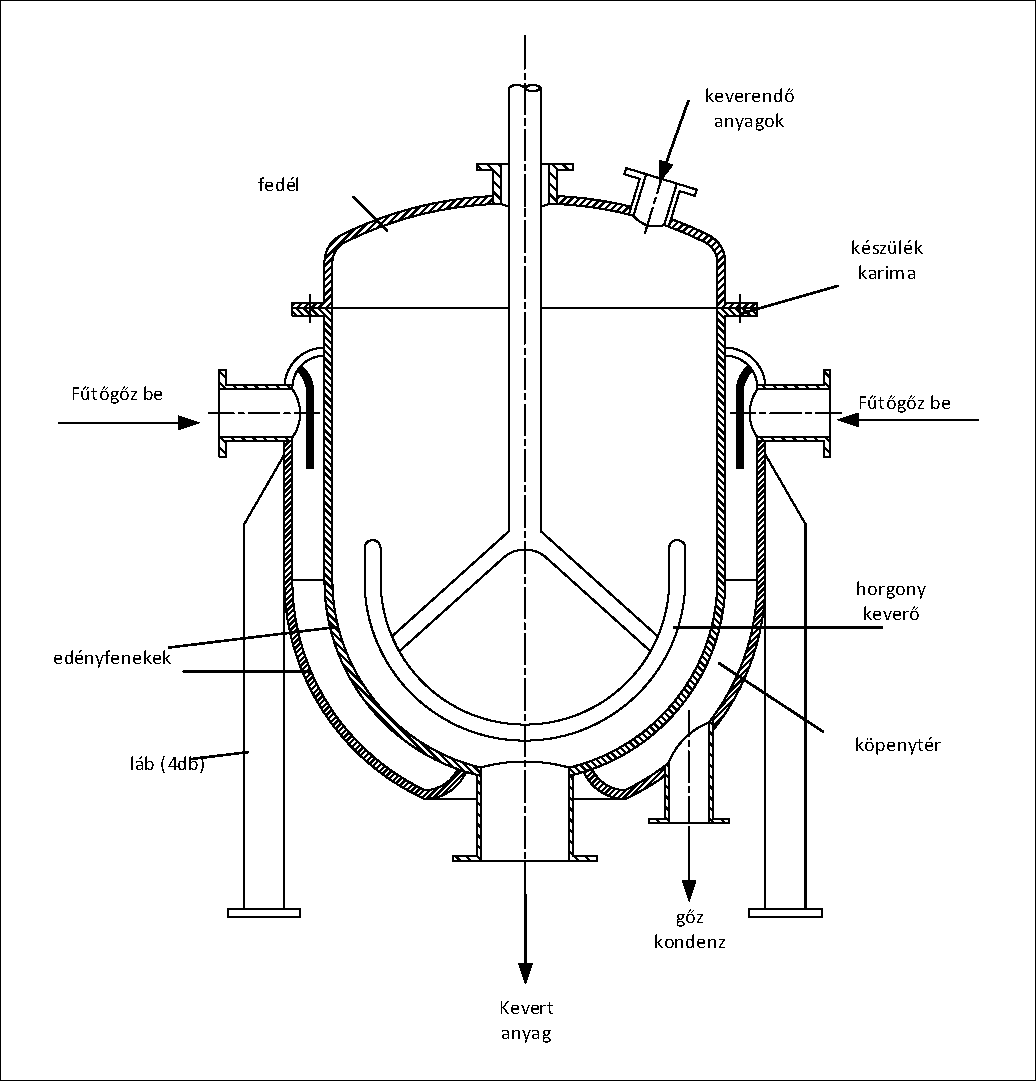
\includegraphics[scale=1, trim=1mm 1mm 1mm 1mm, clip]{kep1}
	\caption{Keverős autókláv}
	\label{kep1356}
\end{figure}




\section{First section}

\section{Second section}

\chapter{Probléma tárgyalása}
Lorem ipsum dolor sit amet,

\section{A Section}

Quisque tristique.

\subsection{A Subsection}
\subsubsection{A Subsection}

Donec urna leo, 

\section{Another Section}

Phasellus nisi quam, 

\section{Alfejezet}
Kezdődik a tényleges szöveg..
És íme, egy képlet
\begin{equation}
Q=\frac{r^4\cdot \pi \cdot \Delta p}{8\cdot \eta\cdot L}
\end{equation}
Kezdődik a tényleges szöveg. Kezdődik a tényleges szöveg, jön a mondanivaló, kifejtése a dolgoknak…. Kezdődik a tényleges szöveg, jön a mondanivaló, kifejtése a dolgoknak….\\

Ilyen egy felsorolás:
\begin{itemize}
	\item első sor
	\item második sor
\end{itemize}
Kezdődik a tényleges szöveg. Kezdődik a tényleges szöveg, jön a mondanivaló, kifejtése a dolgoknak…. Kezdődik a tényleges szöveg, jön a mondanivaló, kifejtése a dolgoknak….\\

És íme, még egy képlet
\begin{equation}\label{egyenlet1}
Q=\frac{r^4\cdot \pi \cdot \Delta p}{8\cdot \eta\cdot L}
\end{equation}

A \ref{egyenlet1}. összefüggés az \cite{fpgaadatlap} szerzőtől származik.
\backmatter
\chapter{Összefoglalás}
\appendix

\chapter{A Melléklet}
\fi

\renewcommand{\refname}{Irodalomjegyzék}
\begin{thebibliography}{9}
    \bibitem{fpgaadatlap} \href{https://datasheet.octopart.com/LCMXO2-4000HC-4MG132I-Lattice-Semiconductor-datasheet-12584740.pdf}{A MachXO2 FPGA család adatlapja }
	 \bibitem{EEPROM} \href{https://ww1.microchip.com/downloads/en/DeviceDoc/doc0670.pdf}{A AT24C256 EEPROM adatlapja }
	\bibitem{FLASH} \href{https://ww1.microchip.com/downloads/en/DeviceDoc/doc0670.pdf}{A W25Q64FV FLASH adatlapja }
\end{thebibliography}





\end{document}